% Created 2015-05-17 Sun 22:16
\documentclass[9pt,b5paper]{article}
\usepackage{graphicx}
\usepackage{xcolor}
\usepackage{xeCJK}
\setCJKmainfont{SimSun}
\usepackage{longtable}
\usepackage{float}
\usepackage{textcomp}
\usepackage{geometry}
\geometry{left=0cm,right=0cm,top=0cm,bottom=0cm}
\usepackage{multirow}
\usepackage{multicol}
\usepackage{listings}
\usepackage{algorithm}
\usepackage{algorithmic}
\usepackage{latexsym}
\usepackage{natbib}
\usepackage{fancyhdr}
\usepackage[xetex,colorlinks=true,CJKbookmarks=true,linkcolor=blue,urlcolor=blue,menucolor=blue]{hyperref}


\lstset{language=c++,numbers=left,numberstyle=\tiny,basicstyle=\ttfamily\small,tabsize=4,frame=none,escapeinside=``,extendedchars=false,keywordstyle=\color{blue!70},commentstyle=\color{red!55!green!55!blue!55!},rulesepcolor=\color{red!20!green!20!blue!20!}}
\author{deepwaterooo}
\date{\today}
\title{QThread Re-entrant \& thread-Safe}
\hypersetup{
  pdfkeywords={},
  pdfsubject={},
  pdfcreator={Emacs 24.3.1 (Org mode 8.2.7c)}}
\begin{document}

\maketitle
\tableofcontents


\section{QT的信号与槽机制}
\label{sec-1}
\subsection{概述}
\label{sec-1-1}
\begin{itemize}
\item 所有从 QObject或其子类(例如Qwidget)派生的类都能够包含信号和槽。当对象改变其状态时,信号就由该对象发射(emit)出去,这就是对象所要做的全部事情,它不知道另一端是谁在接收这个信号。这就是真正的信息封装,它确保对象被当作一个真正的软件组件来使用。槽用于接收信号,但它们是普通的对象成员函数。一个槽并不知道是否有任何信号与自己相连接。而且,对象并不了解具体的通信机制。
\item 你可以将很多信号与单个的槽进行连接,也可以将单个的信号与很多的槽进行连接,甚至于将一个信号与另外一个信号相连接也是可能的,这时无论第一个信号什么时候发射系统都将立刻发射第二个信号。总之,信号与槽构造了一个强大的部件编程机制。
\end{itemize}
\subsection{信号}
\label{sec-1-2}
\begin{itemize}
\item 信号-槽机制完全独立于任何GUI事件循环。只有当所有的槽返回以后发射函数(emit)才返回。如果存在多个槽与某个信号相关联,那么,当这个信号被发射时,这些槽将会一个接一个地执行,但是它们执行的顺序将会是随机的、不确定的,我们不能人为地指定哪个先执行、哪 个后执行。
\item 信号的声明是在头文件中进行的,QT的signals关键字指出进入了信号声明区,随后即可 声明自己的信号。例如,下面定义了三个信号:

\lstset{language=java,label= ,caption= ,numbers=none}
\begin{lstlisting}
signals:  
    void mySignal();  
    void mySignal(int x);  
    void mySignalParam(int x,int y);
\end{lstlisting}

\item 在上面的定义中,signals是QT的关键字,而非C/C++的。接下来的一行void mySignal() 定义了信号mySignal,这个信号没有携带参数;接下来的一行void mySignal(int x)定义了重名信号mySignal,但是它携带一个整形参数,这有点类似于C++中的虚函数。从形式上讲信号的声明与普通的C++函数是一样的,但是信号却没有函数体定义,另外,信号的返回 类型都是void,不要指望能从信号返回什么有用信息。
\item 信号由moc自动产生,它们不应该在.cpp文件中实现。
\end{itemize}
\subsection{槽}
\label{sec-1-3}
\begin{itemize}
\item 槽是普通的C++成员函数,可以被正常调用,它们唯一的特殊性就是很多信号可以与其相关联。当与其关联的信号被发射时,这个槽就会被调用。槽可以有参数,但槽的参数不能有缺省值。
\item 既然槽是普通的成员函数,因此与其它的函数一样,它们也有存取权限。槽的存取权限决定了谁能够与其相关联。同普通的C++成员函数一样,槽函数也分为三种类型,即public slots、private slots和protected slots。
\begin{itemize}
\item public slots:在这个区内声明的槽意味着任何对象都可将信号与之相连接。这对于组件编程非常有用,你可以创建彼此互不了解的对象,将它们的信号与槽进行连接以便信息能够正确的传递。
\item protected slots:在这个区内声明的槽意味着当前类及其子类可以将信号与之相连接。这适用于那些槽,它们是类实现的一部分,但是其界面接口却面向外部。
\item private slots:在这个区内声明的槽意味着只有类自己可以将信号与之相连接。这适用于联系非常紧密的类。
\end{itemize}
\item 槽也能够声明为虚函数,这也是非常有用的。
\item 槽的声明也是在头文件中进行的。例如,下面声明了三个槽:
\lstset{language=java,label= ,caption= ,numbers=none}
\begin{lstlisting}
public slots:   
    void mySlot();   
    void mySlot(int x);   
    void mySignalParam(int x,int y);
\end{lstlisting}
\end{itemize}
\subsection{信号与槽的关联}
\label{sec-1-4}
\begin{itemize}
\item 通过调用QObject对象的connect函数来将某个对象的信号与另外一个对象的槽函数相关联,这样当发射者发射信号时,接收者的槽函数将被调用。该函数的定义如下:
\lstset{language=java,label= ,caption= ,numbers=none}
\begin{lstlisting}
bool QObject::connect ( const QObject * sender, const char * signal,  
                        const QObject * receiver, const char * member ) [static]
\end{lstlisting}

\item 这个函数的作用就是将发射者sender对象中的信号signal与接收者receiver中的member槽函数联系起来。当指定信号signal时必须使用QT的宏SIGNAL(),当指定槽函数时必须使用宏SLOT()。如果发射者与接收者属于同一个对象的话,那么在connect调用中接收者参数可以省略。
\item 一个信号甚至能够与另一个信号相关联,看下面的例子:

\lstset{language=java,label= ,caption= ,numbers=none}
\begin{lstlisting}
class MyWidget : public QWidget {  
public:  
    MyWidget();  
    //    ...  
signals:  
    void aSignal();  
    //    ...  
private:  
    //    ...  
    QPushButton *aButton;  
};  

MyWidget::MyWidget() {  
    aButton = new QPushButton( this );  
    connect(aButton, SIGNAL(clicked()), SIGNAL(aSignal()));  
}
\end{lstlisting}

\item 在上面的构造函数中,MyWidget创建了一个私有的按钮aButton,按钮的单击事件产生的信号clicked()与另外一个信号aSignal ()进行了关联。这样一来,当信号clicked()被发射时,信号aSignal()也接着被发射。当然,你也可以直接将单击事件与某个私有的槽函数相关联,然后在槽中发射aSignal()信号,这样的话似乎有点多余。
\item 当信号与槽没有必要继续保持关联时,我们可以使用disconnect函数来断开连接。其定义如下:
\lstset{language=java,label= ,caption= ,numbers=none}
\begin{lstlisting}
bool QObject::disconnect ( const QObject * sender, const char * signal,  
                           const Object * receiver, const char * member ) [static]
\end{lstlisting}

\item 这个函数断开发射者中的信号与接收者中的槽函数之间的关联。
\item 有三种情况必须使用disconnect()函数:
\begin{itemize}
\item 断开与某个对象相关联的任何对象。这似乎有点不可理解,事实上,当我们在某个对象中定义了一个或者多个信号,这些信号与另外若干个对象中的槽相关联,如果我们要切断这些关联的话,就可以利用这个方法,非常之简洁。
\lstset{language=java,label= ,caption= ,numbers=none}
\begin{lstlisting}
disconnect( myObject, 0, 0, 0 )
\end{lstlisting}

或者
\lstset{language=java,label= ,caption= ,numbers=none}
\begin{lstlisting}
myObject->disconnect()
\end{lstlisting}
\item 断开与某个特定信号的任何关联。
\lstset{language=java,label= ,caption= ,numbers=none}
\begin{lstlisting}
disconnect( myObject, SIGNAL(mySignal()), 0, 0 )
\end{lstlisting}

或者

\lstset{language=java,label= ,caption= ,numbers=none}
\begin{lstlisting}
myObject->disconnect( SIGNAL(mySignal()) )
\end{lstlisting}
\item 断开两个对象之间的关联。
\lstset{language=java,label= ,caption= ,numbers=none}
\begin{lstlisting}
disconnect( myObject, 0, myReceiver, 0 )
\end{lstlisting}
或者
\lstset{language=java,label= ,caption= ,numbers=none}
\begin{lstlisting}
myObject->disconnect( myReceiver )
\end{lstlisting}
\end{itemize}
\item 在disconnect函数中0可以用作一个通配符,分别表示任何信号、任何接收对象、接收对象中的任何槽函数。但是发射者sender不能为0,其它三个参数的值可以等于0。
\end{itemize}
\subsection{元对象工具}
\label{sec-1-5}
\begin{itemize}
\item 元对象编译器moc(meta object compiler)对C++文件中的类声明进行分析并产生用于初始化元对象的C++代码,元对象包含全部信号和槽的名字以及指向这些函数的指针。
\item moc读C++源文件,如果发现有Q$_{\text{OBJECT宏声明的类,它就会生成另外一个C}}$++源文件,这个新生成的文件中包含有该类的元对象代码。例如,假设我们有一个头文件mysignal.h,在这个文件中包含有信号或槽的声明,那么在编译之前 moc 工具就会根据该文件自动生成一个名为mysignal.moc.h的C++源文件并将其提交给编译器;类似地,对应于mysignal.cpp文件moc 工具将自动生成一个名为mysignal.moc.cpp文件提交给编译器。
\item 元对象代码是signal/slot机制所必须的。用moc产生的C++源文件必须与类实现一起进行编译和连接,或者用\#include语句将其包含到类的源文件中。moc并不扩展\#include或者\#define宏定义,它只是简单的跳过所遇到的任何预处理指令。
\end{itemize}
\subsection{examples}
\label{sec-1-6}
\begin{itemize}
\item \lstset{language=java,label= ,caption= ,numbers=none}
\begin{lstlisting}
//tsignal.h  
class TsignalApp : public QMainWindow {  
    Q_OBJECT  

    //信号声明区  
signals:  
    //声明信号mySignal()  
    void mySignal();  
    //声明信号mySignal(int)  
    void mySignal(int x);  
    //声明信号mySignalParam(int, int)  
    void mySignalParam(int x, int y);  
 
    //槽声明区  
public slots:  
    //声明槽函数mySlot()  
    void mySlot();  
    //声明槽函数mySlot(int)  
    void mySlot(int x);  
    //声明槽函数mySignalParam (int,int)  
    void mySignalParam(int x, int y);  
};
 
//tsignal.cpp  
TsignalApp::TsignalApp()   {  
    //将信号mySignal()与槽mySlot()相关联  
    connect(this, SIGNAL(mySignal()), SLOT(mySlot()));  
    //将信号mySignal(int)与槽mySlot(int)相关联  
    connect(this, SIGNAL(mySignal(int)), SLOT(mySlot(int)));  
    //将信号mySignalParam(int, int)与槽mySlotParam(int, int)相关联  
    connect(this, SIGNAL(mySignalParam(int, int)), SLOT(mySlotParam(int, int)));  
}  
 
// 定义槽函数mySlot()  
void TsignalApp::mySlot()   {  
    QMessageBox::about(this, "Tsignal",  "This is a signal/slot sample without parameter.");  
}  
 
// 定义槽函数mySlot(int)  
void TsignalApp::mySlot(int x)   {  
    QMessageBox::about(this, "Tsignal",  "This is a signal/slot sample with one parameter.");  
}  
 
// 定义槽函数mySlotParam(int, int)  
void TsignalApp::mySlotParam(int x, int y)   {  
    char s[256];  
    sprintf(s, "x:%d y:%d", x, y);  
    QMessageBox::about(this, "Tsignal",  s);  
}  
void TsignalApp::slotFileNew()   {  
    //发射信号mySignal()  
    emit mySignal();  
    //发射信号mySignal(int)  
    emit mySignal(5);  
    //发射信号mySignalParam(5,100)  
    emit mySignalParam(5, 100);  
}
\end{lstlisting}
\end{itemize}
\subsection{应注意的问题}
\label{sec-1-7}
\begin{itemize}
\item 1.信号与槽的效率是非常高的,但是同真正的回调函数比较起来,由于增加了灵活性,因此在速度上还是有所损失,当然这种损失相对来说是比较小的,通过在一台i586-133的机器上测试是10微秒(运行Linux),可见这种机制所提供的简洁性、灵活性还是值得的。但如果我们要追求高效率的话,比如在实时系统中就要尽可能的少用这种机制。
\item 2.信号与槽机制与普通函数的调用一样,如果使用不当的话,在程序执行时也有可能产生死循环。因此,在定义槽函数时一定要注意避免间接形成无限循环,即在槽中再次发射所接收到的同样信号。例如,在前面给出的例子中如果在mySlot()槽函数中加上语句emit mySignal()即可形成死循环。
\item 3.如果一个信号与多个槽相联系的话,那么,当这个信号被发射时,与之相关的槽被激活的顺序将是随机的。
\item 4. 宏定义不能用在signal和slot的参数中。
\begin{itemize}
\item 既然moc工具不扩展\#define,因此,在signals和slots中携带参数的宏就不能正确地工作,如果不带参数是可以的。例如,下面的例子中将带有参数的宏SIGNEDNESS(a)作为信号的参数是不合语法的:
\lstset{language=java,label= ,caption= ,numbers=none}
\begin{lstlisting}
#ifdef ultrix  
#define SIGNEDNESS(a) unsigned a  
#else  
#define SIGNEDNESS(a) a  
#endif  
class Whatever : public QObject {  
    signals:  
    void someSignal( SIGNEDNESS(a) );  
};
\end{lstlisting}
\end{itemize}
\item 5.构造函数不能用在signals或者slots声明区域内。
\begin{itemize}
\item 的确,将一个构造函数放在signals或者slots区内有点不可理解,无论如何,不能将它们放在private slots、protected slots或者public slots区内。下面的用法是不合语法要求的:
\lstset{language=java,label= ,caption= ,numbers=none}
\begin{lstlisting}
class SomeClass : public QObject {  
    Q_OBJECT  
public slots:  
    SomeClass( QObject *parent, const char *name )  
        : QObject( parent, name ) {} // 在槽声明区内声明构造函数不合语法  
};
\end{lstlisting}
\end{itemize}
\item 6. 函数指针不能作为信号或槽的参数。
\begin{itemize}
\item 例如,下面的例子中将void (\textbf{applyFunction)(QList}, void*)作为参数是不合语法的:
\lstset{language=java,label= ,caption= ,numbers=none}
\begin{lstlisting}
class someClass : public QObject   {  
    Q_OBJECT  
public slots:  
    void apply(void (*applyFunction)(QList*, void*), char*); // 不合语法  
};
\end{lstlisting}
\item 你可以采用下面的方法绕过这个限制:
\lstset{language=java,label= ,caption= ,numbers=none}
\begin{lstlisting}
typedef void (*ApplyFunctionType)(QList*, void*);  
class someClass : public QObject {  
    Q_OBJECT  
    public slots:  
    void apply( ApplyFunctionType, char *);  
};
\end{lstlisting}
\end{itemize}
\item 7. 信号与槽不能有缺省参数。
\begin{itemize}
\item 既然signal->slot绑定是发生在运行时刻,那么,从概念上讲使用缺省参数是困难的。下面的用法是不合理的:
\lstset{language=java,label= ,caption= ,numbers=none}
\begin{lstlisting}
class SomeClass : public QObject {  
    Q_OBJECT  
public slots:  
    void someSlot(int x = 100); // 将x的缺省值定义成100,在槽函数声明中使用是错误的  
};
\end{lstlisting}
\end{itemize}
\item 8. 信号与槽也不能携带模板类参数。
\begin{itemize}
\item 如果将信号、槽声明为模板类参数的话,即使moc工具不报告错误,也不可能得到预期的结果。 例如,下面的例子中当信号发射时,槽函数不会被正确调用:
\lstset{language=java,label= ,caption= ,numbers=none}
\begin{lstlisting}
public slots:  
    void MyWidget::setLocation (pair location);  
public signals:
    void MyObject::moved (pair location);
\end{lstlisting}
\item 但是,你可以使用typedef语句来绕过这个限制。如下所示:
\lstset{language=java,label= ,caption= ,numbers=none}
\begin{lstlisting}
typedef pair IntPair;  
public slots:  
    void MyWidget::setLocation (IntPair location);  
public signals:  
    void MyObject::moved (IntPair location);
\end{lstlisting}
\item 这样使用的话,你就可以得到正确的结果。
\end{itemize}
\item 9. 嵌套的类不能位于信号或槽区域内,也不能有信号或者槽。
\begin{itemize}
\item 例如,下面的例子中,在class B中声明槽b()是不合语法的,在信号区内声明槽b()也是不合语法的。
\lstset{language=java,label= ,caption= ,numbers=none}
\begin{lstlisting}
class A {  
    Q_OBJECT  
public:  
    class B {  
    public slots:  // 在嵌套类中声明槽不合语法  
    void b();  
    };  
signals:  
    class B {  
        // 在信号区内声明嵌套类不合语法  
        void b();  
    }:  
};
\end{lstlisting}
\end{itemize}
\item 10.友元声明不能位于信号或者槽声明区内。相反,它们应该在普通C++的private、protected或者public区内进行声明。下面的例子是不合语法规范的:
\lstset{language=java,label= ,caption= ,numbers=none}
\begin{lstlisting}
class someClass : public QObject {  
    Q_OBJECT  
signals: //信号定义区  
    friend class ClassTemplate; // 此处定义不合语法
};
\end{lstlisting}
\end{itemize}

\section{Qt多线程之可重入与线程安全}
\label{sec-2}
\begin{itemize}
\item \textbf{可重入} : 假如一个类的任何函数在此类的多个不同的实例上,可以被多个线程同时调用,那么这个类被称为是“可重入”的。
\item \textbf{线程安全} : 假如不同的线程作用在同一个实例上仍可以正常工作,那么称之为“线程安全”的。
\end{itemize}
\subsection{QObject可重入性}
\label{sec-2-1}
\begin{itemize}
\item QObject是可重入的。它的大多数非GUI子类,像QTimer,QTcpSocket,QUdpSocket,QHttp,QFtp,QProcess也是可重入的,在多个线程中同时使用这些类是可能的。
\item 需要注意的是,这些类被设计成在一个单线程中创建与使用,因此,在一个线程中创建一个对象,而在另外的线程中调用它的函数,这样的行为不能保证工作良好。
\item 有三种约束需要注意:
\begin{itemize}
\item QObject的孩子总是应该在它父亲被创建的那个线程中创建。这意味着,你绝不应该传递QThread对象作为另一个对象的父亲(因为QThread对象本身会在另一个线程中被创建)
\item 事件驱动对象仅仅在单线程中使用。明确地说,这个规则适用于"定时器机制“与”网格模块“,举例来讲,你不应该在一个线程中开始一个定时器或是连接一个套接字,当这个线程不是这些对象所在的线程。
\item 你必须保证在线程中创建的所有对象在你删除QThread前被删除。这很容易做到:你可以run()函数运行的栈上创建对象。
\end{itemize}
\item 尽管QObject是可重入的,但GUI类,特别是QWidget与它的所有子类都是不可重入的。它们仅用于主线程。正如前面提到过的,QCoreApplication::exec()也必须从那个线程中被调用。实践上,不会在别的线程中使用GUI类,它们工作在主线程上,把一些耗时的操作放入独立的工作线程中,当工作线程运行完成,把结果在主线程所拥有的屏幕上显示。
\end{itemize}
\subsection{逐线程事件循环}
\label{sec-2-2}
\begin{itemize}
\item 每个线程可以有它的事件循环,初始线程开始它的事件循环需使用QCoreApplication::exec(),别的线程开始它的事件循环需要用QThread::exec().像QCoreApplication一样,QThread提供了exit(int)函数,一个quit() slot。
\item 线程中的事件循环,使得线程可以使用那些需要事件循环的非GUI 类(如,QTimer,QTcpSocket,QProcess)。也可以把任何线程的signals连接到特定线程的slots,也就是说信号-槽机制是可以跨线程使用的。对于在QApplication之前创建的对象,QObject::thread()返回0,这意味着主线程仅为这些对象处理投递事件,不会为没有所属线程的对象处理另外的事件。
\item 可以用 \textbf{QObject::moveToThread()} 来改变它和它孩子们的线程亲缘关系,假如对象有父亲,它不能移动这种关系。在另一个线程(而不是创建它的那个线程)中delete QObject对象是不安全的。除非你可以保证在同一时刻对象不在处理事件。可以用QObject::deleteLater(),它会投递一个DeferredDelete事件,这会被对象线程的事件循环最终选取到。
\item 假如没有事件循环运行,事件不会分发给对象。举例来说,假如你在一个线程中创建了一个QTimer对象,但从没有调用过exec(),那么QTimer就不会发射它的timeout()信号.对deleteLater()也不会工作。(这同样适用于主线程)。你可以手工使用线程安全的函数QCoreApplication::postEvent(),在任何时候,给任何线程中的任何对象投递一个事件,事件会在那个创建了对象的线程中通过事件循环派发。事件过滤器在所有线程中也被支持,不过它限定被监视对象与监视对象生存在同一线程中。类似地,QCoreApplication::sendEvent(不是postEvent()),仅用于在调用此函数的线程中向目标对象投递事件。
\end{itemize}
\subsection{从别的线程中访问QObject子类}
\label{sec-2-3}
\begin{itemize}
\item QObject和所有它的子类是非线程安全的。这包括整个的事件投递系统。需要牢记的是,当你正从别的线程中访问对象时,事件循环可以向你的QObject子类投递事件。假如你调用一个不生存在当前线程中的QObject子类的函数时,你必须用mutex来保护QObject子类的内部数据,否则会遭遇灾难或非预期结果。像其它的对象一样,QThread对象生存在创建它的那个线程中---不是当QThread::run()被调用时创建的那个线程。一般来讲,在你的QThread子类中提供slots是不安全的,除非你用mutex保护了你的成员变量。
\item 另一方面,你可以安全的从QThread::run()的实现中发射信号,因为信号发射是线程安全的。
\end{itemize}
\subsection{跨线程的信号-槽}
\label{sec-2-4}
\begin{itemize}
\item Qt支持三种类型的信号-槽连接:
\begin{itemize}
\item 1,直接连接,当signal发射时,slot立即调用。此slot在发射signal的那个线程中被执行(不一定是接收对象生存的那个线程(?))
\item 2,队列连接,当控制权回到对象属于的那个线程的事件循环时,slot被调用。此slot在接收对象生存的那个线程中被执行
\item 3,自动连接(缺省),假如信号发射与接收者在同一个线程中,其行为如直接连接,否则,其行为如队列连接。
\end{itemize}
\item 连接类型可能通过以向connect()传递参数来指定。注意的是,当发送者与接收者生存在不同的线程中,而事件循环正运行于接收者的线程中,使用直接连接是不安全的。同样的道理,调用生存在不同的线程中的对象的函数也是不是安全的。QObject::connect()本身是线程安全的。
\end{itemize}
\subsection{多线程与隐含共享}
\label{sec-2-5}
\begin{itemize}
\item Qt为它的许多值类型使用了所谓的隐含共享(implicit sharing)来优化性能。原理比较简单,共享类包含一个指向共享数据块的指针,这个数据块中包含了真正原数据与一个引用计数。把深拷贝转化为一个浅拷贝,从而提高了性能。这种机制在幕后发生作用,程序员不需要关心它。如果深入点看,假如对象需要对数据进行修改,而引用计数大于1,那么它应该先detach()。以使得它修改不会对别的共享者产生影响,既然修改后的数据与原来的那份数据不同了,因此不可能再共享了,于是它先执行深拷贝,把数据取回来,再在这份数据上进行修改。例如:

\lstset{language=java,label= ,caption= ,numbers=none}
\begin{lstlisting}
void QPen::setStyle(Qt::PenStyle style){  
     detach();           // detach from common data  
     d->stylestyle = style;   // set the style member  
}  
void QPen::detach(){   
    if (d->ref != 1) {  
         ...             // perform a deep copy  
     }  
}
\end{lstlisting}
\item 一般认为,隐含共享与多线程不太和谐,因为有引用计数的存在。对引用计数进行保护的方法之一是使用mutex,但它很慢,Qt早期版本没有提供一个满意的解决方案。从4.0开始,隐含共享类可以安全地跨线程拷贝,如同别的值类型一样。它们是 \textbf{完全可重入} 的。隐含共享真的是"implicit"。它使用汇编语言实现了原子性引用计数操作,这比用mutex快多了。
\item 假如你在多个线程中同进访问相同对象,你也需要用mutex来串行化访问顺序,就如同其他可重入对象那样。总的来讲,隐含共享真的给”隐含“掉了,在多线程程序中,你可以把它们看成是一般的,非共享的,可重入的类型,这种做法是安全的。
\end{itemize}

\section{QThread使用方法: QThread中的slots在那个线程中执行?}
\label{sec-3}
Reference: \url{http://mobile.51cto.com/symbian-268690.htm}
\subsection{QThread::run}
\label{sec-3-1}
\begin{itemize}
\item run 对于线程的作用相当于main函数对于应用程序。它是线程的入口,run的开始和结束意味着线程的开始和结束。 原文如下: The run() implementation is for a thread what the main() entry point is for the application. All code executed in a call stack that starts in the run() function is executed by the new thread, and the thread finishes when the function returns.  
\lstset{language=java,label= ,caption= ,numbers=none}
\begin{lstlisting}
class Thread : public QThread {       
    Q_OBJECT
public:       
    Thread(QObject* parent = 0)
        : QThread(parent) {
    }
public slots:       
    void slot() { ... }
signals:       
    void sig();
protected:       
    void run() { ...}
};    

int main(int argc, char** argv) {
    ...
    Thread thread;
    ...
}
\end{lstlisting}
\item 对照前面的定理,run函数中的代码时确定无疑要在次线程中运行的,那么其他的呢?比如 slot 是在次线程还是主线程中运行?
\end{itemize}
\subsection{QObject::connect}
\label{sec-3-2}
\subsubsection{three connection types}
\label{sec-3-2-1}
\begin{enumerate}
\item 自动连接(Auto Connection)
\label{sec-3-2-1-1}
\begin{itemize}
\item 这是默认设置
\item 如果发送者和接收者处于同一线程,则等同于直接连接
\item 如果发送者和接受者位于不同线程,则等同于队列连接
\item 也就是这说,只存在下面两种情况
\end{itemize}
\item 直接连接(Direct Connection)
\label{sec-3-2-1-2}
\begin{itemize}
\item 当信号发射时,槽函数将直接被调用。
\item 无论槽函数所属对象在哪个线程,槽函数都在发射者所在线程执行。
\end{itemize}
\item 队列连接(Queued Connection)
\label{sec-3-2-1-3}
\begin{itemize}
\item 当控制权回到接受者所在线程的事件循环时,槽函数被调用。
\item 槽函数在接收者所在线程执行。
\end{itemize}
\end{enumerate}
\subsubsection{explain by examples}
\label{sec-3-2-2}
\begin{itemize}
\item 不妨继续拿前面的例子来看,slot 函数是在主线程还是次线程中执行呢?
\item 定理二强调两个概念:发送者所在线程 和 接收者所在线程。而 slot 函数属于我们在main中创建的对象 thread,即thread属于主线程
\begin{itemize}
\item 队列连接告诉我们:槽函数在接受者所在线程执行。即 slot 将在主线程执行
\item 直接连接告诉我们:槽函数在发送者所在线程执行。发送者在那个线程呢??不定!
\item 自动连接告诉我们:二者不在同一线程时,等同于队列连接。即 slot 在主线程执行
\end{itemize}
\item 要彻底理解这几句话,你可能需要看 \textbf{Qt meta-object系统} 和 \textbf{Qt event系统} 
\begin{itemize}
\item QThread 是用来管理线程的,它所处的线程和它管理的线程并不是同一个东西
\item QThread 所处的线程,就是执行 QThread t(0) 或 QThread * t=new QThread(0) 的线程。也就是咱们这儿的主线程
\item QThread 管理的线程,就是 run 启动的线程。也就是次线程
\item 因为QThread的对象在主线程中,所以他的slot函数会在主线程中执行,而不是次线程。除非:QThread 对象在次线程中
\item slot和信号是直接连接,且信号所属对象在次线程中
\end{itemize}
\item 但上两种解决方法都不好,因为QThread不是这么用的(Bradley T. Hughes)
\end{itemize}
\subsection{主线程(信号) \textasciitilde{} QThread(槽)}
\label{sec-3-3}
\begin{itemize}
\item 这是Qt Manual 和 例子中普遍采用的方法。 但由于manual没说槽函数是在主线程执行的,所以不少人都认为它应该是在次线程执行了。
\begin{itemize}
\item 定义一个 Dummy 类,用来发信号
\item 定义一个 Thread 类,用来接收信号
\item 重载 run 函数,目的是打印 threadid
\end{itemize}
\lstset{language=java,label= ,caption= ,numbers=none}
\begin{lstlisting}
#include <QtCore/QCoreApplication>   
#include <QtCore/QObject>   
#include <QtCore/QThread>   
#include <QtCore/QDebug>

class Dummy : public QObject {       
    Q_OBJECT
public:     
    Dummy(){}
public slots:
    void emitsig() {
        emit sig();       
    }
signals:
    void sig();   
};    

class Thread : public QThread {      
    Q_OBJECT
public:       
    Thread(QObject* parent = 0)
        : QThread(parent) {
        //moveToThread(this);
    }   
public slots:
    void slot_main () {           
        qDebug() << "from thread slot_main:" << currentThreadId();       
    }
protected:
    void run() {           
        qDebug() << "thread thread:" << currentThreadId();           
        exec();       
    }   
};
    
//#include "main.moc"
int main(int argc, char *argv[]) {       
    QCoreApplication a(argc, argv);       
    qDebug() << "main thread:" << QThread::currentThreadId();
    Thread thread;       
    Dummy dummy;      
    QObject::connect(&dummy, SIGNAL(sig()), &thread, SLOT(slot_main()));       
    thread.start();      
    dummy.emitsig();       
    return a.exec();
}
\end{lstlisting}
\item 然后看到结果(具体值每次都变,但结论不变)

\lstset{language=java,label= ,caption= ,numbers=none}
\begin{lstlisting}
main thread:           0x1a40 
from thread slot_main: 0x1a40 
thread thread:         0x1a48 

Mine here:
Starting /home/jenny/480/qt/build-dummyThread-Unnamed-Debug/dummyThread...
main thread:           140534496016256 
from thread slot_main: 140534496016256 
thread thread:         140534421948160
\end{lstlisting}
\item 看到了吧,槽函数的线程和主线程是一样的!
\item 如果你看过Qt自带的例子,你会发现 QThread 中 slot 和 run 函数共同操作的对象,都会用QMutex锁住。为什么?因为slot和run处于不同线程,需要线程间的同步!
\item 如果想让槽函数slot在次线程运行(比如它执行耗时的操作,会让主线程死掉),怎么解决呢?
\item 注意:发送dummy信号是在主线程, 接收者 thread 也在主线程中。 参考我们前面的结论,很容易想到: 将 thread 放到次线程中不就行了 这也是代码中注释掉的 moveToThread(this)所做的,去掉注释,你会发现slot在次线程中运行
\lstset{language=java,label= ,caption= ,numbers=none}
\begin{lstlisting}
main thread:           0x13c0 
thread thread:         0x1de0 
from thread slot_main: 0x1de0 

Mine here: 
Starting /home/jenny/480/qt/build-dummyThread-Unnamed-Debug/dummyThread...
main thread:           140371166443392 
thread thread:         140371092375296 
from thread slot_main: 140371092375296
\end{lstlisting}
\item 这可以工作,但这是 Bradley T. Hughes 强烈批判的用法。推荐的方法后面会给出。
\end{itemize}
\subsection{run中信号与QThread中槽}
\label{sec-3-4}
Reference: \url{http://mobile.51cto.com/symbian-268690_1.htm}
\begin{itemize}
\item examples:
\begin{itemize}
\item 定义一个 Dummy 类,在run中发射它的信号
\item 也可以在run中发射 Thread 中的信号,而不是Dummy(效果完全一样),QThread 定义槽函数,重载run函数
\end{itemize}
\lstset{language=java,label= ,caption= ,numbers=none}
\begin{lstlisting}
#include <QtCore/QCoreApplication>   
#include <QtCore/QObject>   
#include <QtCore/QThread>   
#include <QtCore/QDebug>    

class Dummy : public QObject {       
    Q_OBJECT
public:
    Dummy(QObject* parent = 0)
        : QObject(parent) {}   
public slots:
    void emitsig() {        
        emit sig();    
    }
signals:
    void sig();
};    

class Thread : public QThread {       
    Q_OBJECT
public:      
    Thread(QObject* parent = 0)
        : QThread(parent) {
        //moveToThread(this);
    }   
public slots:
    void slot_thread() {           
        qDebug() << "from thread slot_thread:"  << currentThreadId();
    }   
signals:
    void sig();
protected:
    void run() {           
        qDebug() << "thread thread:" << currentThreadId();          
        Dummy dummy;           
        connect(&dummy, SIGNAL(sig()), this, SLOT(slot_thread()));          
        dummy.emitsig();
        exec();       
    }   
};    

//#include "main.moc"
int main(int argc, char *argv[]) {       
    QCoreApplication a(argc, argv);       
    qDebug() << "main thread:" << QThread::currentThreadId();       
    Thread thread;       
    thread.start();       
    return a.exec();
}
\end{lstlisting}
\item 想看结果么?

\lstset{language=java,label= ,caption= ,numbers=none}
\begin{lstlisting}
main thread:             0x15c0 
thread thread:           0x1750 
from thread slot_thread: 0x15c0

Mine here: 
Starting /home/jenny/480/qt/build-dummyThread-Unnamed-Debug/dummyThread...
main thread:             140388248221568 
thread thread:           140388174153472 
from thread slot_thread: 140388248221568
\end{lstlisting}
\item 其实没悬念,肯定是主线程
\item thread 对象本身在主线程。所以它的槽也在要在主线程执行,如何解决呢?
\begin{itemize}
\item (方法一)前面提了 moveToThread,这儿可以用,而且可以解决问题。当同样,是被批判的对象。
\lstset{language=java,label= ,caption= ,numbers=none}
\begin{lstlisting}
uncomment moveToThread(this); line :
Starting /home/jenny/480/qt/build-dummyThread-Unnamed-Debug/dummyThread...
main thread:             140217092188032 
thread thread:           140217018119936 
from thread slot_thread: 140217018119936
\end{lstlisting}
\item (方法二)注意哦,这儿我们的信号时次线程发出的,对比connect连接方式,会发现:
\begin{itemize}
\item 采用直接连接,槽函数将在次线程(信号发出的线程)执行
\item 这个方法不太好,因为你需要处理slot和它的对象所在线程的同步。需要 QMutex 一类的东西(have \textbf{NOT} tried this method yet\textasciitilde{}!!)
\end{itemize}
\item (方法三)推荐的方法,其实,这个方法太简单,太好用了。定义一个普通的QObject派生类,然后将其对象move到QThread中。使用信号和槽时根本不用考虑多线程的存在。也不用使用QMutex来进行同步,Qt的事件循环会自己自动处理好这个。
\lstset{language=java,label= ,caption= ,numbers=none}
\begin{lstlisting}
#include <QtCore/QCoreApplication>   
#include <QtCore/QObject>   
#include <QtCore/QThread>   
#include <QtCore/QDebug>    

class Dummy : public QObject {       
    Q_OBJECT   
public:
    Dummy(QObject* parent = 0)
        : QObject(parent) {}   
public slots:
    void emitsig() {
        emit sig();       
    }
signals:
    void sig();
};

class Object : public QObject {       
    Q_OBJECT   
public:
    Object(){}
public slots:
    void slot() {    
        qDebug() << "from thread slot:"  << QThread::currentThreadId();       
    }   
};    

//#include "main.moc"
int main(int argc, char *argv[]) {      
    QCoreApplication a(argc, argv);       
    qDebug() << "main thread:" << QThread::currentThreadId();      
    QThread thread;       
    Object obj;       
    Dummy dummy;       
    obj.moveToThread(&thread);      
    QObject::connect(&dummy, SIGNAL(sig()), &obj, SLOT(slot()));      
    thread.start();       
    dummy.emitsig();       
    return a.exec();
}
\end{lstlisting}
\begin{itemize}
\item 结果:恩,slot确实不在主线程中运行(这么简单不值得欢呼么?)

\lstset{language=java,label= ,caption= ,numbers=none}
\begin{lstlisting}
main thread:      0x1a5c
from thread slot: 0x186c 

Mine here: 
Starting /home/jenny/480/qt/build-dummyThread-Unnamed-Debug/dummyThread...
main thread:      139964716550016 
from thread slot: 139964642481920
\end{lstlisting}
\end{itemize}
\end{itemize}
\end{itemize}

\section{QT中关于信号与槽机制的实现原理: 源代码分析}
\label{sec-4}
本文介绍的内容是QT中关于信号与槽机制的实现原理,每个对象都有一个相应的纪录该对象的元对象,关于元对象的类在本文中有所介绍。
\subsection{每个对象都有一个相应的纪录该对象的元对象}
\label{sec-4-1}
关于元对象的类:下面介绍有两种
\subsubsection{QMetaObject类}
\label{sec-4-1-1}
\begin{itemize}
\item \lstset{language=java,label= ,caption= ,numbers=none}
\begin{lstlisting}
/*******************生成元对象需要的输入参数*****************/  
// 类名  
const char * const class_name;  

// 父类名  
QMetaObject *superclass;  

// 记录slot信息  
const QMetaData * const slot_data;   

// 记录槽的个数  
int n_slots;  

// 记录signal信息  
const QMetaData * const signal_data;  

// 记录信号的个数  
int n_signals;

/******************* 元对象类提供的方法**************************/  
int numSlots( bool super = FALSE ) const;   // 返回槽的个数  
int numSignals( bool super = FALSE ) const; // 返回信号的个数  
int findSlot( const char *, bool super = FALSE ) const;   // 查找槽  
int findSignal( const char *, bool super = FALSE ) const; // 查找信号  

// 返回指定位置的槽  
const QMetaData *slot( int index, bool super = FALSE ) const;  

// 返回指定位置的信号  
const QMetaData *signal( int index, bool super = FALSE ) const;  

// 所有槽名字的列表  
QStrList slotNames( bool super = FALSE ) const;  

// 所有信号名字的列表  
QStrList signalNames( bool super = FALSE ) const;  

// 槽的起始索引  
int slotOffset() const;  

// 信号的起始索引  
int signalOffset() const;  

/***********************两个获取类的元对象的方法*****************/  
static QMetaObject *metaObject( const char *class_name );  
static bool hasMetaObject( const char *class_name );
\end{lstlisting}
\end{itemize}
\subsubsection{QMetaData类}
\label{sec-4-1-2}
\lstset{language=java,label= ,caption= ,numbers=none}
\begin{lstlisting}
  // 记录元对象数据for 信号与槽  
struct QMetaData {                                   
    const char *name;       // 名称  
    const QUMethod* method; // 详细描述信息  
    enum Access { Private, Protected, Public };  
    Access access;          // 访问权限  
};
\end{lstlisting}

\subsection{QObject类实现了信号与槽机制}
\label{sec-4-2}
它利用元对象纪录的信息,实现了信号与槽机制.
\subsubsection{信号与槽建立连接的实现}
\label{sec-4-2-1}
\begin{enumerate}
\item 接口函数:
\label{sec-4-2-1-1}
\lstset{language=c++,label= ,caption= ,numbers=none}
\begin{lstlisting}
// 连接  
// 参数(发送对象,信号,接收对象,处理信号的信号/槽)
static bool connect(const QObject *sender, const char *signal,  
                    const QObject *receiver, const char *member );  
bool connect(const QObject *sender, const char *signal,  
             const char *member ) const;

static bool disconnect(const QObject *sender, const char *signal,  
                       const QObject *receiver, const char *member);  
bool disconnect(const char *signal = 0,  
                const QObject *receiver = 0, const char *member = 0 );  
bool disconnect(const QObject *receiver, const char *member = 0 );

// 连接的内部实现  
// (发送对象,信号的索引,接收对象,处理信号的类型,处理信号信号/槽的索引)    
static void connectInternal(const QObject *sender, int signal_index,  
                            const QObject *receiver, int membcode, int member_index );  
static bool disconnectInternal(const QObject *sender, int signal_index,  
                               const QObject *receiver, int membcode, int member_index );
\end{lstlisting}
\item 信号与槽连接的实现原理:
\label{sec-4-2-1-2}
\lstset{language=c++,label= ,caption= ,numbers=none}
\begin{lstlisting}
// 一阶段  
bool QObject::connect(const QObject *sender,   // 发送对象        
                      const char *signal,      // 信号  
                      const QObject *receiver, // 接收对象  
                      const char *member       // 槽  
                      ) { 
    // 检查发送对象,信号,接收对象,槽不为null  
    if ( sender == 0 || receiver == 0 || signal == 0 || member == 0 ) {        
        return false;  
    }
    
    // 获取发送对象的元对象  
    QMetaObject *smeta = sender->metaObject();  
    // 检查信号  
    if ( !check_signal_macro( sender, signal, "connect", "bind" ) )  
        return false;     
    // 获取信号的索引  
    int signal_index = smeta->findSignal( signal, true );  
    if ( signal_index < 0 ) {                // normalize and retry  
        nw_signal = qt_rmWS( signal-1 ); // remove whitespace  
        signal = nw_signal.data()+1;         // skip member type code  
        signal_index = smeta->findSignal( signal, true );  
    }  
    // 如果信号不存在,则退出  
    if ( signal_index < 0  ) {                    // no such signal  
        return false;  
    }  

    // 获取信号的元数据对象  
    const QMetaData *sm = smeta->signal( signal_index, true );  
    // 获取信号名字  
    signal = sm->name;         
    // 获取处理信号的类型(是信号/槽)  
    int membcode = member[0] - '0';        // get member code    // **** membcode
    // 发送信号对象  
    QObject *s = (QObject *)sender;        // we need to change them  
    // 接收信号对象  
    QObject *r = (QObject *)receiver;      //   internally  
    // 获取接收对象的元对象  
    QMetaObject *rrmeta = r->metaObject();  
    int member_index = -1;  

    switch ( membcode ) {                // get receiver member  
    case QSLOT_CODE:// 如果是槽  
        // 获取槽索引  
        member_index = rmeta->findSlot( member, true );  
        if ( member_index < 0 ) {            // normalize and retry  
            nw_member = qt_rmWS(member);     // remove whitespace  
            member = nw_member;  
            member_index = rmeta->findSlot( member, true );  
        }  
        break;  
    case QSIGNAL_CODE:// 如果是信号  
        // 获取信号索引  
        member_index = rmeta->findSignal( member, true );  
        if ( member_index < 0 ) {           // normalize and retry  
            nw_member = qt_rmWS(member);     // remove whitespace  
            member = nw_member;  
            member_index = rmeta->findSignal( member, true );  
        }  
        break;  
    }  
    // 如果接收对象不存在相应的信号或槽,则退出  
    if ( member_index < 0  ) {  
        return false;  
    }  
    // 检查连接的参数(发送的信号,接收对象,处理信号的槽或信号)  
    if ( !s->checkConnectArgs(signal,receiver,member) ) {  
        return false;  
    } else {  
        // 获取处理信号的元数据对象  
        const QMetaData *rm = membcode == QSLOT_CODE ?  
            rmeta->slot( member_index, true ) :  
            rmeta->signal( member_index, true );  
        if ( rm ) {            
            // 建立连接  
            // (发送信号的对象,信号的索引,接收信号的对象,处理信号的类型,处理信号的索引)  
            connectInternal( sender, signal_index, receiver, membcode, member_index );  
        }  
    }  
    return true;  
}  

// 二阶段  
// 建立连接  
// (发送信号的对象,信号的索引,接收信号的对象,处理信号的类型,处理信号的索引)  
void QObject::connectInternal( const QObject *sender, int signal_index,   
                               const QObject *receiver, int membcode, int member_index )   {  
    // 发送信号的对象  
    QObject *s = (QObject*)sender;  
    // 接收信号的对象  
    QObject *r = (QObject*)receiver;  
    // 如果发送对象的连接查询表为null,则建立  
    if ( !s->connections ) {                // create connections lookup table  
        s->connections = new QSignalVec( signal_index+1 );  
        Q_CHECK_PTR( s->connections );  
        s->connections->setAutoDelete( true );  
    }  
    // 获取发送对象的相应信号的连接列表  
    QConnectionList *clist = s->connections->at( signal_index );  
    if ( !clist ) {                         // create receiver list  
        clist = new QConnectionList;  
        Q_CHECK_PTR( clist );  
        clist->setAutoDelete( true );  
        s->connections->insert( signal_index, clist );  
    }  
    QMetaObject *rrmeta = r->metaObject();  
    const QMetaData *rm = 0;  
    switch ( membcode ) {                // get receiver member  
    case QSLOT_CODE:  
        rm = rmeta->slot( member_index, true );  
        break;  
    case QSIGNAL_CODE:  
        rm = rmeta->signal( member_index, true );  
        break;  
    }  
    // 建立连接  
    QConnection *c = new QConnection( r, member_index, rm ? rm->name : "qt_invoke", membcode );  
    Q_CHECK_PTR( c );  
    // 把连接添加到发送对象的连接列表中  
    clist->append( c );  
    // 判断接收对象的发送对象列表是否为null  
    if ( !r->senderObjects ) {               // create list of senders 
        // 建立接收对象的发送对象列表  
        r->senderObjects = new QSenderObjectList;  
    }  
    // 把发送对象添加到发送对象列表中  
    r->senderObjects->append( s );           // add sender to list  
}
\end{lstlisting}

\item 信号发生时激活的操作函数。 激活slot的方法
\label{sec-4-2-1-3}
\lstset{language=java,label= ,caption= ,numbers=none}
\begin{lstlisting}
// 接口:
void QObject::activate_signal( int signal ) {  
#ifndef QT_NO_PRELIMINARY_SIGNAL_SPY  
    if ( qt_preliminary_signal_spy ) {  
    //信号没有被阻塞  
    //信号>=0  
    //连接列表不为空,或者信号对应的连接存在  
    if ( !signalsBlocked() && signal >= 0 &&  
        (!connections || !connections->at( signal )) ) {  
        QUObject o[1];  
        qt_spy_signal( this, signal, o );  
        return;  
    }  
}  
#endif  
    if ( !connections || signalsBlocked() || signal < 0 )  
        return;  
    //获取信号对应的连接列表  
    QConnectionList *clist = connections->at( signal );  
    if ( !clist )  
        return;  
    QUObject o[1];  
    //  
    activate_signal( clist, o );  
}  
 
void QObject::activate_signal( QConnectionList *clist, QUObject *o )   {  
    if ( !clist )  
        return;  
#ifndef QT_NO_PRELIMINARY_SIGNAL_SPY  
    if ( qt_preliminary_signal_spy )  
        qt_spy_signal( this, connections->findRef( clist), o );  
#endif  
    QObject *object;  
    //发送对象列表  
    QSenderObjectList* sol;  
    //旧的发送对象  
    QObject* oldSender = 0;  
    //连接  
    QConnection *c;  
    if ( clist->count() == 1 ) { // save iterator  
        //获取连接  
        c = clist->first();  
        //  
        object = c->object();  
        //获取发送对象列表  
        sol = object->senderObjects;  
        if ( sol ) {  
            //获取旧的发送对象  
            oldSender = sol->currentSender;  
            //  
            sol->ref();  
            //设置新的发送对象  
            sol->currentSender = this;  
        }  
        if ( c->memberType() == QSIGNAL_CODE )//如果是信号,则发送出去  
            object->qt_emit( c->member(), o );  
        else  
            object->qt_invoke( c->member(), o );//如果是槽,则执行  
        //       
        if ( sol ) {  
            //设置恢复为旧的发送对象  
            sol->currentSender = oldSender;  
            if ( sol->deref() )  
                delete sol;  
        }  
    } else {  
        QConnection *cd = 0;  
        QConnectionListIt it(*clist);  
        while ( (c=it.current()) ) {  
            ++it;  
            if ( c == cd )  
                continue;  
            ccd = c;   
            object = c->object();  
            //操作前设置当前发送对象  
            sol = object->senderObjects;  
            if ( sol ) {  
                oldSender = sol->currentSender;  
                sol->ref();  
                sol->currentSender = this;  
            }  
            //如果是信号,则发送出去  
            if ( c->memberType() == QSIGNAL_CODE ){  
                object->qt_emit( c->member(), o );  
            }  
            //如果是槽,则执行  
            else {  
                object->qt_invoke( c->member(), o );  
            }  
            //操作后恢复当前发送对象  
            if (sol ) {  
                sol->currentSender = oldSender;  
                if ( sol->deref() )  
                    delete sol;  
            }  
        } // while  
    }  
}
\end{lstlisting}
\end{enumerate}

\section{正确使用Qt多线程}
\label{sec-5}
Reference: \url{http://my.oschina.net/u/200628/blog/187865}
\subsection{QThread的常见特性}
\label{sec-5-1}
\begin{itemize}
\item run()是线程的入口,就像main()对于应用程序的作用。QThread中对run()的默认实现调用了exec(),从而创建一个QEventLoop对象,由其处理该线程事件队列(每一个线程都有一个属于自己的事件队列)中的事件。简单用代码描述如下:
\lstset{language=java,label= ,caption= ,numbers=none}
\begin{lstlisting}
int QThread::exec() {
    //...
    QEventLoop eventLoop;
    int returnCode = eventLoop.exec();
    //...
    return returnCode;
}

int QEventLoop::exec(ProcessEventsFlags flags) {
    //...
    while (!d->exit) {
        while (!posted_event_queue_is_empty) {
            process_next_posted_event();
        }
    }
    //...
}
\end{lstlisting}
\item 由此可见,exec()在其内部不断做着循环遍历事件队列的工作,调用QThread的quit()或exit()方法使停止工作,尽量不要使用terminate(),该方法过于粗暴,造成资源不能释放,甚至互斥锁还处于加锁状态。
\end{itemize}
\subsection{旧的使用方式}
\label{sec-5-2}
\lstset{language=java,label= ,caption= ,numbers=none}
\begin{lstlisting}
#include "QThread"
#include "QMutexLocker"
#include "QMutex"

class Thread : public QThread {
    Q_OBJECT
public:
    Thread();
    void stop();
private:
    bool m_stopFlag;
    QMutex mutex;
protected:
    void run();
};

Thread::Thread() {
    m_stopFlag = false;
}
  
void Thread::stop() {
    QMutexLocker locker(&mutex);
    m_stopFlag = true;
}
  
void Thread::run() {
    while (1) {
        {
            QMutexLocker locker(&mutex);
            if(m_stopFlag)
                break;
        }
        qDebug() << "This is in thread[" << currentThreadId() << "]." << (int)currentThread();
        sleep(2);
    }
    m_stopFlag = false;
}
\end{lstlisting}
\begin{itemize}
\item 这是qt4.6及之前的使用方法,这种方式本没有什么错误,可以处理我们的绝大多数需求。下面的调用可以看出Thread对象本身工作在主线程下,即使调用的t.stop()方法,它也是工作在主线程下,只有run()范围内的代码工作在次线程中。

\lstset{language=java,label= ,caption= ,numbers=none}
\begin{lstlisting}
int main(int argc, char *argv[]) {
    QCoreApplication a(argc, argv);
    qDebug() << "From main thread: " << QThread::currentThreadId();
    Thread t;
    QObject::connect(&t, SIGNAL(finished()), &a, SLOT(quit()));
    t.start();
    return a.exec();
}
\end{lstlisting}
\end{itemize}
\subsection{推荐的使用方式}
\label{sec-5-3}
\begin{itemize}
\item \lstset{language=java,label= ,caption= ,numbers=none}
\begin{lstlisting}
#include <QtCore>

class Worker : public QObject {
    Q_OBJECT
private slots:
    void onTimeout() {
        qDebug() << "Worker::onTimeout get called from?: " << QThread::currentThreadId();
    }
};
  
//#include "main.moc"
int main(int argc, char *argv[]) {
    QCoreApplication a(argc, argv);
    qDebug() << "From main thread: " << QThread::currentThreadId();
    QThread t;
    QTimer timer;
    Worker worker;
    QObject::connect(&timer, SIGNAL(timeout()), &worker, SLOT(onTimeout()));
    timer.start(1000);
    worker.moveToThread(&t);
    t.start();
    return a.exec();
}
\end{lstlisting}
\item 这是Qt4.7及以后版本推荐的工作方式。其主要特点就是利用Qt的事件驱动特性,将需要在次线程中处理的业务放在独立的模块(类)中,由主线程创建完该对象后,将其移交给指定的线程,且可以将多个类似的对象移交给同一个线程。在这个例子中,信号由主线程的QTimer对象发出,之后Qt会将关联的事件放到worker所属线程的事件队列。由于队列连接的作用,在不同线程间连接信号和槽是很安全的。
\end{itemize}
\subsection{GUI界面假死的处理}
\label{sec-5-4}
\begin{itemize}
\item 在GUI程序中,主线程也叫GUI线程,因为它是唯一被允许执行GUI相关操作的线程。对于一些耗时的操作,如果放在主线程中,就是出现界面无法响应的问题。这种问题的解决一种方式是,把这些耗时操作放到次线程中,还有一种比较简单的方法:在处理耗时操作中频繁调用QApplication::processEvents()。这个函数告诉Qt去处理那些还没有被处理的各类事件,然后再把控制权返还给调用者。

\lstset{language=java,label= ,caption= ,numbers=none}
\begin{lstlisting}
QElapsedTimer et;
et.start();
while(et.elapsed()<300)
    QCoreApplication::processEvents();
\end{lstlisting}
\end{itemize}

\section{QThread related Examples}
\label{sec-6}
\subsection{QMutex}
\label{sec-6-1}
\begin{itemize}
\item \lstset{language=java,label= ,caption= ,numbers=none}
\begin{lstlisting}
class MyClass {
 public:
    void doStuff(int c) {
        mutex.lock();
        a = c;
        b = c * 2;
        mutex.unlock();
    }
 private:
    QMutex mutex;
    int a;
    int b;
};
\end{lstlisting}
\end{itemize}
\subsection{QReadWriteLock}
\label{sec-6-2}
\begin{itemize}
\item this one is not working, try some other\ldots{}.
\lstset{language=java,label= ,caption= ,numbers=none}
\begin{lstlisting}
#include <QApplication>
#include <QPushButton>
#include <QWaitCondition>

QWaitCondition mycond;

class Worker : public QPushButton, public QThread {
    Q_OBJECT
 public:
    Worker(QWidget *parent = 0, const char *name = 0)
        : QPushButton(parent, name) {
        setText("start working");
        //connect(this, SIGNAL(clicked()), SLOT(slotClicked()));
        QThread.start();
    }
    public slots:
        void slotClicked() {
            mycond.wakeOne();
        }
 protected:
        void run() {
            while (TRUE) {
                qApp->lock();
                setCaption("waiting");
                qApp->unlock();

                mycond.wait();

                qApp->lock();
                setCaption("working!");
                qApp->unlock();
                do_complicated_thing();
            }
        }
};

int main(int argc, char *argv[]) {
    QApplication app(argc, argv);
    Worker firstworker(0, "worker");
    app.setMainWidget(&worker);
    worker.show();
    return app.exec();
}
\end{lstlisting}
\item codes parts
\lstset{language=java,label= ,caption= ,numbers=none}
\begin{lstlisting}
QReadWriteLock lock;
void ReaderThread::run() {
    // ...
    lock.lockForRead();
    read_file();
    lock.unlock();
    //...
}
void WriterThread::run() {
    // ...
    lock.lockForWrite();
    write_file();
    lock.unlock();
    // ...
}
\end{lstlisting}
\end{itemize}

\subsection{Consumer Producer: QWaitCondition}
\label{sec-6-3}
\begin{itemize}
\item consumer.h
\lstset{language=java,label= ,caption= ,numbers=none}
\begin{lstlisting}
#ifndef CONSUER_H
#define CONSUER_H

#include <QObject>
#include <QThread>
#include <QTime>
#include <stdio.h>
#include <QWaitCondition>
#include <QMutex>
#include "producer.h"

extern const int DataSize;
extern const int BufferSize;

extern char buffer[BufferSize];
extern QWaitCondition bufferNotEmpty;
extern QWaitCondition bufferNotFull;
extern QMutex mutex;
extern int numUsedBytes;

class Consumer : public QThread {
    Q_OBJECT
 public:
    void run() {
        for (int i = 0; i < DataSize; ++i) {
            mutex.lock();
            if (numUsedBytes == 0)
                bufferNotEmpty.wait(&mutex);
            mutex.unlock();

            fprintf(stderr, "%c", buffer[i % BufferSize]);

            mutex.lock();
            --numUsedBytes;
            bufferNotFull.wakeAll();
            mutex.unlock();
        }
        fprintf(stderr, "\n");
    }

    virtual ~Consumer() {};
};

#endif
\end{lstlisting}
\item producer.h
\lstset{language=java,label= ,caption= ,numbers=none}
\begin{lstlisting}
#ifndef PRODUCER_H
#define PRODUCER_H

#include <QObject>
#include <QThread>
#include <QTime>
#include <QWaitCondition>
#include <QMutex>

const int DataSize = 1000;
const int BufferSize = 200;

extern char buffer[BufferSize];
extern QWaitCondition bufferNotEmpty;
extern QWaitCondition bufferNotFull;
extern QMutex mutex;
extern int numUsedBytes;

class Producer : public QThread {
    Q_OBJECT
 public:
    void run() {
        qsrand(QTime(0, 0, 0).secsTo(QTime::currentTime()));
        for (int i = 0; i < DataSize; ++i) {
            mutex.lock();
            if (numUsedBytes == BufferSize)
                bufferNotFull.wait(&mutex);
            mutex.unlock();

            buffer[i % BufferSize] = "aeiu"[(int)qrand() % 4];

            mutex.lock();
            ++numUsedBytes;
            bufferNotEmpty.wakeAll();
            mutex.unlock();
        }
    }
    virtual ~Producer() {};
};

#endif
\end{lstlisting}
\item main.cpp
\lstset{language=java,label= ,caption= ,numbers=none}
\begin{lstlisting}
#include <QtCore>
#include <stdio.h>
#include "mainwindow.h"
#include "producer.h"
#include "consumer.h"

extern const int DataSize;
extern const int BufferSize;

char buffer[BufferSize];
QWaitCondition bufferNotEmpty;
QWaitCondition bufferNotFull;
QMutex mutex;
int numUsedBytes = 0;

int main(int argc, char *argv[]) {
    QCoreApplication app(argc, argv);
    Producer producer;
    Consumer consumer;
    producer.start();
    consumer.start();
    producer.wait();
    consumer.wait();
    return 0;
}
\end{lstlisting}
\end{itemize}

\subsection{Consumer Producer: QSemaphore}
\label{sec-6-4}
\begin{itemize}
\item producer
\lstset{language=java,label= ,caption= ,numbers=none}
\begin{lstlisting}
const int DataSize = 100000;
const int BufferSize = 8192;
char buffer[BufferSize];

QSemaphore freeBytes(BufferSize);
QSemaphore usedBytes;

class Producer : public QThread {
public:
    void run() {
        qsrand(QTime(0,0,0).secsTo(QTime::currentTime()));
        for (int i = 0; i < DataSize; ++i) {
            freeBytes.acquire();
            buffer[i % BufferSize] = "zero"[(int)qrand() % 4];
            usedBytes.release();
        }
    }
};
\end{lstlisting}
\item consumer
\lstset{language=java,label= ,caption= ,numbers=none}
\begin{lstlisting}
#include "producer.h"

class Consumer : public QThread {
public:
    void run() {
        for (int i = 0; i < DataSize; ++i) {
            usedBytes.acquire();
            fprintf(stderr, "%c", buffer[i % BufferSize]);
            freeBytes.release();
        }
        fprintf(stderr, "\n");
    }
};
\end{lstlisting}
\item main.cpp
\lstset{language=java,label= ,caption= ,numbers=none}
\begin{lstlisting}
extern const int DataSize;
extern const int BufferSize;
extern char buffer[BufferSize];

QWaitCondition bufferNotEmpty;
QWaitCondition bufferNotFull;
QMutex mutex;
int numUsedBytes = 0;

int main(int argc, char *argv[]) {
    QCoreApplication app(argc, argv);
    Producer producer;
    Consumer consumer;
    producer.start();
    consumer.start();
    producer.wait();
    consumer.wait();
    return 0;
}
\end{lstlisting}
\end{itemize}

\subsection{Mandelbrotset}
\label{sec-6-5}
\begin{itemize}
\item renderthread.h

\lstset{language=java,label= ,caption= ,numbers=none}
\begin{lstlisting}
#ifndef RENDERTHREAD_H
#define RENDERTHREAD_H

#include <QMutex>
#include <QSize>
#include <QThread>
#include <QWaitCondition>
#include <QImage>

class RenderThread : public QThread {
    Q_OBJECT
 public:
    RenderThread(QObject *parent = 0);
    ~RenderThread();
    void render(double centerX, double centerY, double scaleFactor, QSize resultSize);
 signals:
    void renderedImage(const QImage &image, double scaleFactor);
 protected:
    void run();
 private:
    uint rgbFromWaveLength(double wave);
    QMutex mutex;
    QWaitCondition condition;
    double centerX;
    double centerY;
    double scaleFactor;
    QSize resultSize;
    bool restart;
    bool abort;
    enum {ColormapSize = 512};
    uint colormap[ColormapSize];
};

#endif
\end{lstlisting}
\item renderthread.cpp

\lstset{language=java,label= ,caption= ,numbers=none}
\begin{lstlisting}
#include <QtGui>
#include <math.h>
#include "renderthread.h"

RenderThread::RenderThread(QObject *parent)
    : QThread(parent) {
    restart = false;
    abort = false;
    for (int i = 0; i < ColormapSize; i++)
        colormap[i] = rgbFromWaveLength(380.0 + (i * 400.0 / ColormapSize));
}

void RenderThread::render(double centerX, double centerY, double scaleFactor, QSize resultSize) {
    QMutexLocker locker(&mutex);
    this->centerX = centerX;
    this->centerY = centerY;
    this->scaleFactor = scaleFactor;
    this->resultSize = resultSize;
    if (!isRunning()) {
        start(LowPriority);
    } else {
        restart = true;
        condition.wakeOne();
    }
}

void RenderThread::run() {
    forever {
        mutex.lock();
        QSize resultSize = this->resultSize;
        double scaleFactor = this->scaleFactor;
        double centerX = this->centerX;
        double centerY = this->centerY;
        mutex.unlock();
        int halfWidth = resultSize.width() / 2;
        int halfHeight = resultSize.height() / 2;
        QImage image(resultSize, QImage::Format_RGB32);
        const int NumPasses = 8;
        int pass = 0;
        while (pass < NumPasses) {
            const int MaxIterations = (1 << (2 * pass + 6)) + 32;
            const int Limit = 4;
            bool allBlack = true;
            for (int y = -halfHeight; y < halfHeight; y++) {
                if (restart) break;
                if (abort) return;
                uint *scanLine = reinterpret_cast<uint*>(image.scanLine(y + halfHeight));
                double ay = centerY + (y * scaleFactor);
                for (int x = -halfWidth; x < halfWidth; x++) {
                    double ax = centerX + (x * scaleFactor);
                    double a1 = ax;
                    double b1 = ay;
                    int numIterations = 0;
                    do {
                        ++numIterations;
                        double a2 = (a1 * a1) - (b1 * b1) + ax;
                        double b2 = (2 * a1 * b1) + ay;
                        if ((a2 * a2) + (b1 * b1) > Limit) break;
                    } while (numIterations < MaxIterations);
                    if (numIterations < MaxIterations) {
                        *scanLine++ = colormap[numIterations % ColormapSize];
                        allBlack = false;
                    } else {
                        *scanLine++ = qRgb(0, 0, 0);
                    }
                }
            }
            if (allBlack && pass == 0) {
                pass = 4;
            } else {
                if (!restart)
                    emit renderedImage(image, scaleFactor);
                ++pass;
            }
        }
        mutex.lock();
        if (!restart) {
            condition.wait(&mutex);
        }
        restart = false;
        mutex.unlock();
    }
}

uint RenderThread::rgbFromWaveLength(double wave) {
    double r = 0.0;
    double g = 0.0;
    double b = 0.0;
    if (wave >= 380.0 && wave <= 440.0) {
        r = -1.0 * (wave - 440.0) / (440.0 - 380.0);
        b = 1.0;
    } else if (wave >= 440.0 && wave <= 490.0) {
        g = (wave - 440.0) / (490.0 - 440.0);
        b = 1.0;
    } else if (wave >= 490.0 && wave <= 510.0) {
        g = 1.0;
        b = -1.0 * (wave - 510.0) / (510.0 - 490.0);
    } else if (wave >= 510.0 && wave <= 580.0) {
        r = (wave - 510.0) / (580.0 - 510.0);
        g = 1.0;
    } else if (wave >= 580.0 && wave <= 645.0) {
        r = 1.0;
        g = -1.0 * (wave - 645.0) / (645.0 - 580.0);
    } else if (wave >= 645.0 && wave <= 780.0) {
        r = 1.0;
    }
    double s = 1.0;
    if (wave > 700.0) {
        s = 0.3 + 0.7 * (780.0 - wave) / (780.0 - 700.0);
    } else {
        s = 0.3 + 0.7 * (wave - 380.0) / (420.0 - 380.0);
    }
    r = pow(r * s, 0.8);
    g = pow(g * s, 0.8);
    b = pow(b * s, 0.8);
    return qRgb(int(r * 255), int(g * 255), int(b * 255));
}

RenderThread::~RenderThread() {
    mutex.lock();
    abort = true;
    condition.wakeOne();
    mutex.unlock();
    wait();
}
\end{lstlisting}
\item Mandelbrotwidget.h

\lstset{language=java,label= ,caption= ,numbers=none}
\begin{lstlisting}
#ifndef MANDELBROTWIDGET_H
#define MANDELBROTWIDGET_H

#include <QPixmap>
#include <QWidget>
#include "renderthread.h"

class MandelbrotWidget : public QWidget {
    Q_OBJECT
 public:
    MandelbrotWidget(QWidget *parent = 0);
 protected:
    void paintEvent(QPaintEvent event);
    void resizeEvent(QResizeEvent *event);
    void keyPressEvent(QKeyEvent *event);
    void wheelEvent(QWheelEvent *event);
    void mousePressEvent(QMouseEvent *event);
    void mouseMoveEvent(QMouseEvent *event);
    void mouseReleaseEvent(QMouseEvent *event);
    private slots:
        void updatePixmap(const QImage &image, double scaleFactor);
 private:
        void zoom(double zoomFactor);
        void scroll(int deltaX, int deltaY);
        RenderThread thread;
        QPixmap pixmap;
        QPoint pixmapOffset;
        QPoint lastDragPos;
        double centerX;
        double centerY;
        double pixmapScale;
        double curScale;
};

#endif
\end{lstlisting}
\item Mandelbrotwidget.cpp

\lstset{language=java,label= ,caption= ,numbers=none}
\begin{lstlisting}
#include <QtGui>
#include <math.h>
#include "mandelbrotwidget.h"

const double DefaultCenterX = -0.637011f;
const double DefaultCenterY = -0.0395159f;
const double DefaultScale = 0.00403897f;
const double ZoomInFactor = 0.8f;
const double ZoomOutFactor = 1 / ZoomInFactor;
const int ScrollStep = 20;

MandelbrotWidget::MandelbrotWidget(QWidget *parent)
    : QWidget(parent) {
    centerX = DefaultCenterX;
    centerY = DefaultCenterY;
    pixmapScale = DefaultScale;
    curScale = DefaultScale;
    qRegisterMetaType<QImage>("QImage");
    connect(&thread, SIGNAL(renderedImage(const QImage &, double)),
            this, SLOT(updatePixmap(const QImage &, double)));
    setWindowTitle(tr("Mandelbrot"));
    setCursor(Qt::CrossCursor);
    resize(550, 400);
}

void MandelbrotWidget::paintEvent(QPaintEvent event) {
    QPainter painter(this);
    painter.fillRect(rect(), Qt::black);
    if (pixmap.isNull()) {
        painter.setPen(Qt::white);
        painter.drawText(rect(), Qt::AlignCenter,
                         tr("Rendering initial image, please wait..."));
        return;
    }
    if (curScale == pixmapScale) {
        painter.drawPixmap(pixmapOffset, pixmap);
    } else {
        double scaleFactor = pixmapScale / curScale;
        int newWidth = int(pixmap.width() * scaleFactor);
        int newHeight = int(pixmap.height() * scaleFactor);
        int newX = pixmapOffset.x() + (pixmap.width() - newWidth) / 2;
        int newY = pixmapOffset.y() + (pixmap.height() - newHeight) / 2;
        painter.save();
        painter.translate(newX, newY);
        painter.scale(scaleFactor, scaleFactor);
        QRectF exposed = painter.matrix().inverted().mapRect(rect().adjusted(-1, -1, 1, 1));
        painter.drawPixmap(exposed, pixmap, exposed);
        painter.restore();
    }
    QString text = tr("Use mouse wheel or the '+' and '-' keys to zoom."
                      "Press and hold left mouse button to scroll.");
    QFontMetrics metrics = painter.fontMetrics();
    int textWidth = metrics.width(text);
    painter.setPen(Qt::NoPen);
    painter.setBrush(QColor(0, 0, 0, 127));
    painter.drawRect((width() - textWidth) / 2 - 5, 0, textWidth + 10, metrics.lineSpacing() + 5);
    painter.setPen(Qt::white);
    painter.drawText((width() - textWidth) / 2, metrics.leading() + metrics.ascent(), text);
}

void MandelbrotWidget::resizeEvent(QResizeEvent *event) {
    thread.render(centerX, centerY, curScale, size());
}

void MandelbrotWidget::keyPressEvent(QKeyEvent *event) {
    switch (event->key()) {
    case Qt::Key_Plus:
        zoom(ZoomInFactor);
        break;
    case Qt::Key_Minus:
        zoom(ZoomOutFactor);
        break;
    case Qt::Key_Left:
        scroll(-ScrollStep, 0);
        break;
    case Qt::Key_Right:
        scroll(+ScrollStep, 0);
        break;
    case Qt::Key_Down:
        scroll(0, -ScrollStep);
        break;
    case Qt::Key_Up:
        scroll(0, +ScrollStep);
        break;
    default:
        QWidget::keyPressEvent(event);
    }
}

void MandelbrotWidget::wheelEvent(QWheelEvent *event) {
    int numDegrees = event->delta() / 8;
    double numSteps = numDegrees / 15.0f;
    zoom(pow(ZoomInFactor, numSteps));
}

void MandelbrotWidget::mousePressEvent(QMouseEvent *event) {
    if (event->button() == Qt::LeftButton) {
        lastDragPos = event->pos();
    }
}

void MandelbrotWidget::mouseMoveEvent(QMouseEvent *event) {
    if (event->buttons() & Qt::LeftButton) {
        pixmapOffset += event->pos() - lastDragPos;
        lastDragPos = event->pos();
        update();
    }
}

void MandelbrotWidget::mouseReleaseEvent(QMouseEvent *event) {
    if (event->button() == Qt::LeftButton) {
        pixmapOffset += event->pos() - lastDragPos;
        lastDragPos = QPoint();
        int deltaX = (width() - pixmap.width()) / 2 - pixmapOffset.x();
        int deltaY = (height() - pixmap.height()) / 2 - pixmapOffset.y();
        scroll(deltaX, deltaY);
    }
}

void MandelbrotWidget::updatePixmap(const QImage &image, double scaleFactor) {
    if (!lastDragPos.isNull()) 
        return;
    pixmap = QPixmap::fromImage(image);
    pixmapOffset = QPoint();
    lastDragPos = QPoint();
    pixmapScale = scaleFactor;
    update();
}

void MandelbrotWidget::zoom(double zoomFactor) {
    curScale *= zoomFactor;
    update();
    thread.render(centerX, centerY, curScale, size());
}

void MandelbrotWidget::scroll(int deltaX, int deltaY) {
    centerX += deltaX * curScale;
    centerY += deltaY * curScale;
    update();
    thread.render(centerX, centerY, curScale, size());
}
\end{lstlisting}

\item main.cpp

\lstset{language=java,label= ,caption= ,numbers=none}
\begin{lstlisting}
#include "mainwindow.h"
#include <QApplication>
#include "mandelbrotwidget.h"

int main(int argc, char *argv[]) {
    QApplication a(argc, argv);
    MandelbrotWidget widget;
    widget.show();
    return a.exec();
}
\end{lstlisting}
\end{itemize}

\section{Linux下 QT 实现串口通讯小实例}
\label{sec-7}
\url{http://mobile.51cto.com/symbian-270754.htm}
\begin{itemize}
\item thread.h

\lstset{language=java,label= ,caption= ,numbers=none}
\begin{lstlisting}
class Thread : public QThread {     
    Q_OBJECT     
public:     
    Thread();     
    char buf[128];     
    volatile bool stopped;     
    volatile bool write_rs;     
    volatile bool read_rs;     
protected:     
    virtual void run();     
};
\end{lstlisting}
\item thread.cpp

\lstset{language=java,label= ,caption= ,numbers=none}
\begin{lstlisting}
#include "thread.h"     
#include <sys/types.h>     
#include <sys/stat.h>     
#include <fcntl.h>     
#include <termios.h>    //串口用到的     
#include <stdio.h>     
#include <stdlib.h>     
#include <unistd.h>     
#include <strings.h>     

#define BAUDRATE B9600     
#define RS_DEVICE "/dev/ttyS0"       //串口0     

//#define RS_DEVICE "/dev/ttySAC1"       //串口1     

Thread::Thread() {}                                                 //析构     

void Thread::run() {         //这就是线程的具体工作了     
    int fd, c = 0, res;     
    struct termios oldtio, newtio;     //termios结构是用来保存波特率、字符大小等     

    printf("start...\n");     
    fd = open(RS_DEVICE, O_RDWR|O_NOCTTY);     //以读写方式打开串口。不控制TTY     
    if (fd < 0) {         
        perror("Got fd < 0 error here");     
        exit(1);                             //失败退出     
    }
    
    printf("Open...\n");     
    tcgetattr(fd, &oldtio);             //保存当前设置到oldtio     
    bzero(&newtio, sizeof(newtio));     //清除newtio结构,并重新对它的成员设置如下    
    newtio.c_cflag = BAUDRATE|CS8|CLOCAL|CREAD;  //9600、8位、忽略DCD信号、启用接收装置     
    newtio.c_iflag |= IGNPAR;                    //忽略奇偶     
    newtio.c_oflag = 0;     
    newtio.c_lflag = 0;     
    newtio.c_cc[VMIN] = 0;     
    newtio.c_cc[VTIME] = 100;                   //在规定时间(VTIME)内读取(VMIN)个字符;     
    tcflush(fd, TCIFLUSH);                    //清除所有队列在串口的输入与输出;     
    tcsetattr(fd, TCSANOW, &newtio);           //把我们的设置写入termios
    
    while (stopped) {     // stopped 为 0 时将退出线程     
        if (write_rs) {   // write_rs 为 1 时把字符串从串口中输出     
            write_rs = 0;     
            write(fd, "QtEmbedded-4.5.1", 16);  //向串口中写入字符,通过串口调试助手可看到QtEmbedded-4.5.1这个字符     
        }     
        if (read_rs) {                          //read_rs 为 1 时读取,并存在buf     
            read_rs = 0;     
            res = read(fd, buf, 10);     //读取串口的数据到buf     
            buf[res] = 0;     
            emit finished();                      //读完后发一个信号     
        }     
    }     

    printf("Close...\n");     
    tcsetattr(fd, TCSANOW, &oldtio);      //重新设置回原来的     
    close(fd);     
    quit();     
}
\end{lstlisting}
\item mainwindow.h

\lstset{language=java,label= ,caption= ,numbers=none}
\begin{lstlisting}
#include "ui_mainwindow.h"    //奇怪?这个头文件从哪里来的?呵呵,刚才用designer做的mainwindow.ui文件,经过make后会生成这个头文件,     
#include "thread.h"           //把我们前面定义的线程包含进来     

class MainWindow : public QMainWindow, public Ui::MainWindow {  //多继承     
    Q_OBJECT     
public:     
    MainWindow(QWidget *parent=0);     
public slots:     
    void writeThread();     
    void readThread();     
    void closeThread();     
    void display();    
private:     
    Thread *yy;     
};
\end{lstlisting}
\item mainwindow.cpp

\lstset{language=java,label= ,caption= ,numbers=none}
\begin{lstlisting}
MainWindow::MainWindow(QWidget *parent)     
    :QMainWindow(parent) {     
    setupUi(this);     
    yy = new Thread;     
    yy->start();          //启动线程     
    yy->stopped=1;        //初始化变量     
    yy->write_rs=0;     
    yy->read_rs=0;     
    connect(writeButton, SIGNAL(clicked()), this, SLOT(writeThread()));      //信号与槽     
    connect(readButton, SIGNAL(clicked()), this, SLOT(readThread()));     
    connect(closeButton, SIGNAL(clicked()), this, SLOT(closeThread()));     
    connect(yy, SIGNAL(finished()), this, SLOT(display()));      //前面线程读完了不是发一个信号么,这个信号就是发到这个槽     
}

void MainWindow::display() {     
    dis_label->setText(yy->buf);     //读到的在dis_label显示,dis_label就是我们前面designer放的标签,显示buf中的内容     
}     

void MainWindow::writeThread() {  //前面线程都是根据stopped、write_rs、read_rs的状态来工作的^_^      
    yy->write_rs = 1;     
}    

void MainWindow::readThread() {     
    yy->read_rs = 1;     
}     

void MainWindow::closeThread() {     
    yy->stopped = 0;     
}
\end{lstlisting}
\item main.cpp

\lstset{language=java,label= ,caption= ,numbers=none}
\begin{lstlisting}
int main(int argc,char *argv[]) {     
    QApplication app(argc,argv);     
    MainWindow mw;     
    mw.show();     
    return app.exec();     
}
\end{lstlisting}
\end{itemize}

\section{another examples}
\label{sec-8}
\begin{itemize}
\item TextDevice.h    
\lstset{language=java,label= ,caption= ,numbers=none}
\begin{lstlisting}
#ifndef TEXTDEVICE_H    
#define TEXTDEVICE_H    

#include <QThread>    
#include <QString>    
#include <QMutex>     

class TextDevice : public QThread {     
    Q_OBJECT     
public:     
    TextDevice();     
    void run();     
    void stop();     
public slots:     
    void write(const QString& text);     
private:     
    int m_count;     
    QMutex m_mutex;     
};    

#endif // TEXTDEVICE_H
\end{lstlisting}

\item TextDevice.cpp    
\lstset{language=java,label= ,caption= ,numbers=none}
\begin{lstlisting}
#include <QMutexLocker>    
#include <QDebug>    
#include <QString>    
#include "textdevice.h"     

TextDevice::TextDevice() {     
    m_count = 0;     
}     

void TextDevice::run() {     
    exec();     
}     

void TextDevice::stop() {     
    quit();     
}     

void TextDevice::write(const QString& text) {     
    QMutexLocker locker(&m_mutex);     
    qDebug() << QString("Call %1: %2").arg(m_count++).arg(text);     
}
\end{lstlisting}

\item TextThread.h    
\lstset{language=java,label= ,caption= ,numbers=none}
\begin{lstlisting}
#ifndef TEXTTHREAD_H    
#define TEXTTHREAD_H    

#include <QThread>    
#include <QString>     

class TextThread : public QThread {     
    Q_OBJECT     
public:     
    TextThread(const QString& text);     
    void run();     
    void stop();     
signals:     
    void writeText(const QString&);     
private:     
    QString m_text;     
    bool m_stop;     
};    

#endif // TEXTTHREAD_H
\end{lstlisting}

\item TextThread.cpp    
\lstset{language=java,label= ,caption= ,numbers=none}
\begin{lstlisting}
#include "textthread.h"     

TextThread::TextThread(const QString& text) : QThread() {     
    m_text = text;     
    m_stop = false;     
}     

void TextThread::stop() {     
    m_stop = true;     
}     

void TextThread::run() {     
    while(!m_stop) {     
        emit writeText(m_text);     
        sleep(1);     
    }     
}
\end{lstlisting}

\item main.cpp    
\lstset{language=java,label= ,caption= ,numbers=none}
\begin{lstlisting}
#include <QApplication>    
#include <QMessageBox>    
#include "textdevice.h"    
#include "textthread.h"     
    
int main(int argc, char** argv) {     

    QApplication app(argc, argv);     
    //启动线程     

    TextDevice device;     
    TextThread foo("foo"), bar("bar");     

    //把两个线程使用signal/slot连接起来     
    QObject::connect(&foo, SIGNAL(writeText(const QString&)), &device, SLOT(write(const QString&)));     
    QObject::connect(&bar, SIGNAL(writeText(const QString&)), &device, SLOT(write(const QString&)));     

    //启动线程     
    foo.start();     
    bar.start();     
    device.start();     

    QMessageBox::information(0, "Threading", "Close me to stop.");     
    //停止线程     
    foo.stop();     
    bar.stop();     
    device.stop();     

    //等待线程结束     
    device.wait();     
    foo.wait();     
    bar.wait();     

    return 0;     
}
\end{lstlisting}
\end{itemize}

\section{volatile}
\label{sec-9}
\url{http://hedengcheng.com/?p=725}

volatile: (The stopped variable is declared) volatile because it is accessed from different threads and we want to be sure that it is freshly read every time it is needed. If we ommitted the volatile keyword, the compiler might optimized access to the variable, possibly leading to incorrect results. 
\subsection{Volatile:易变的}
\label{sec-9-1}
\subsubsection{测试用例一:非Volatile变量}
\label{sec-9-1-1}
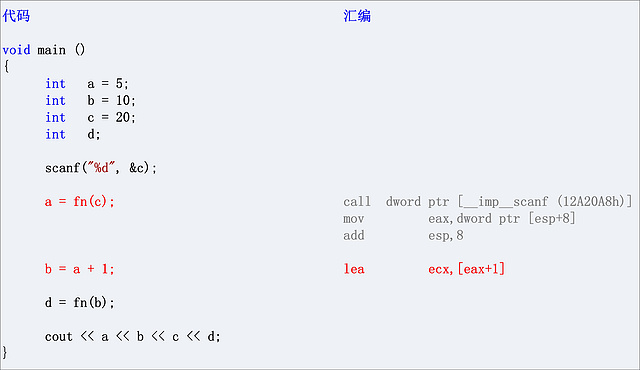
\includegraphics[width=.9\linewidth]{../pic/v1.jpg}
\begin{itemize}
\item b = a + 1;这条语句,对应的汇编指令是:lea ecx, [eax + 1]。由于变量a,在前一条语句a = fn(c)执行时,被缓存在了寄存器eax中,因此b = a + 1;语句,可以直接使用仍旧在寄存器eax中的a,来进行计算,对应的也就是汇编:[eax + 1]。
\end{itemize}
\subsubsection{测试用例二:Volatile变量}
\label{sec-9-1-2}
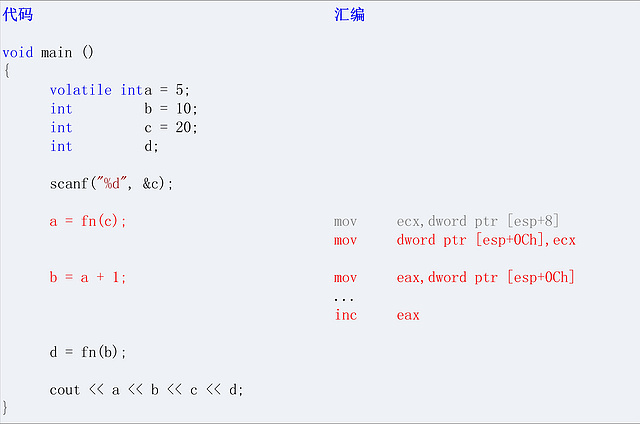
\includegraphics[width=.9\linewidth]{../pic/v2.jpg}
\begin{itemize}
\item 与测试用例一唯一的不同之处,是变量a被设置为volatile属性,一个小小的变化,带来的是汇编代码上很大的变化。a = fn(c)执行后,寄存器ecx中的a,被写回内存:mov dword ptr [esp+0Ch], ecx。然后,在执行b = a + 1;语句时,变量a有重新被从内存中读取出来:mov eax, dword ptr [esp + 0Ch],而不再直接使用寄存器ecx中的内容。
\end{itemize}
\subsubsection{结论}
\label{sec-9-1-3}
\begin{itemize}
\item 易变性。所谓的易变性,在汇编层面反映出来,就是两条语句,下一条语句不会直接使用上一条语句对应的volatile变量的寄存器内容,而是重新从内存中读取。
\end{itemize}
\subsection{Volatile:不可优化的}
\label{sec-9-2}
\subsubsection{测试用例三:非Volatile变量}
\label{sec-9-2-1}
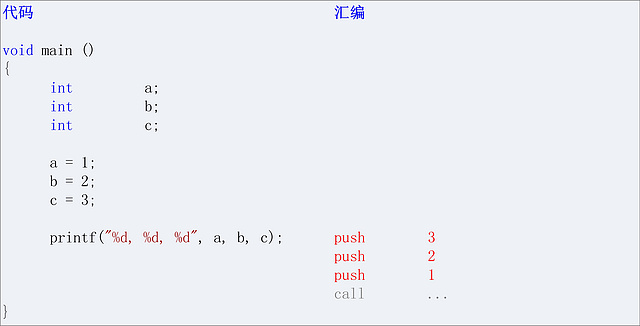
\includegraphics[width=.9\linewidth]{../pic/v3.jpg}
  -在这个用例中,非volatile变量a,b,c全部被编译器优化掉了 (optimize out),因为编译器通过分析,发觉a,b,c三个变量是无用的,可以进行常量替换。最后的汇编代码相当简介,高效率。
\subsubsection{测试用例四:Volatile变量}
\label{sec-9-2-2}
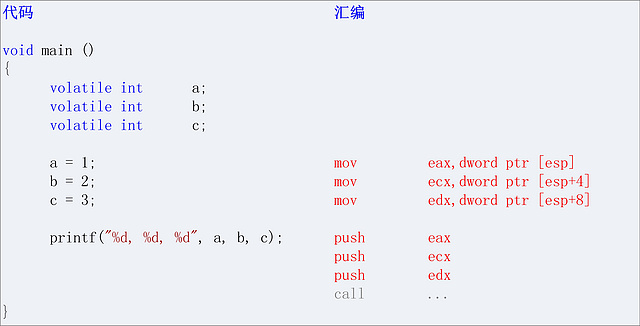
\includegraphics[width=.9\linewidth]{../pic/v4.jpg}
  -测试用例四,与测试用例三类似,不同之处在于,a,b,c三个变量,都是volatile变量。这个区别,反映到汇编语言中,就是三个变量仍旧存在,需要将三个变量从内存读入到寄存器之中,然后再调用printf()函数。
\subsubsection{结论}
\label{sec-9-2-3}
\begin{itemize}
\item “不可优化”特性。volatile告诉编译器,不要对我这个变量进行各种激进的优化,甚至将变量直接消除,保证程序员写在代码中的指令,一定会被执行。相对于前面提到的第一个特性:”易变”性,”不可优化”特性可能知晓的人会相对少一些。但是,相对于下面提到的C/C++ Volatile的第三个特性,无论是”易变”性,还是”不可优化”性,都是Volatile关键词非常流行的概念。
\end{itemize}
\subsection{Volatile:顺序性}
\label{sec-9-3}
\begin{itemize}
\item C/C++ Volatile关键词前面提到的两个特性,让Volatile经常被解读为一个为多线程而生的关键词:一个全局变量,会被多线程同时访问/修改,那么线程内部,就不能假设此变量的不变性,并且基于此假设,来做一些程序设计。当然,这样的假设,本身并没有什么问题,多线程编程,并发访问/修改的全局变量,通常都会建议加上Volatile关键词修饰,来防止C/C++编译器进行不必要的优化。但是,很多时候,C/C++ Volatile关键词,在多线程环境下,会被赋予更多的功能,从而导致问题的出现。
\item 回到本文背景部分我的那篇微博,我的这位朋友,正好犯了一个这样的问题。其对C/C++ Volatile关键词的使用,可以抽象为下面的伪代码:

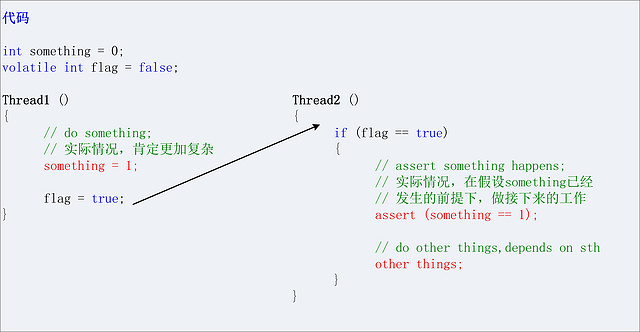
\includegraphics[width=.9\linewidth]{../pic/v5.jpg}
\item 这段伪代码,声明另一个Volatile的flag变量。一个线程(Thread1)在完成一些操作后,会修改这个变量。而另外一个线程(Thread2),则不断读取这个flag变量,由于flag变量被声明了volatile属性,因此编译器在编译时,并不会每次都从寄存器中读取此变量,同时也不会通过各种激进的优化,直接将if (flag \texttt{= true)改写为if (false =} true)。只要flag变量在Thread1中被修改,Thread2中就会读取到这个变化,进入if条件判断,然后进入if内部进行处理。在if条件的内部,由于flag == true,那么假设Thread1中的something操作一定已经完成了,在基于这个假设的基础上,继续进行下面的other things操作。
\item 通过将flag变量声明为volatile属性,很好的利用了本文前面提到的C/C++ Volatile的两个特性:”易变”性;”不可优化”性。按理说,这是一个对于volatile关键词的很好应用,而且看到这里的朋友,也可以去检查检查自己的代码,我相信肯定会有这样的使用存在。
\item 但是,这个多线程下看似对于C/C++ Volatile关键词完美的应用,实际上却是有大问题的。问题的关键,就在于前面标红的文字:由于flag = true,那么假设Thread1中的something操作一定已经完成了。flag \texttt{= true,为什么能够推断出Thread1中的something一定完成了?其实既然我把这作为一个错误的用例,答案是一目了然的:这个推断不能成立,你不能假设看到flag =} true后,flag = true;这条语句前面的something一定已经执行完成了。这就引出了C/C++ Volatile关键词的第三个特性:顺序性。
\item 同样,为了说明C/C++ Volatile关键词的”顺序性”特征,下面给出三个简单的用例 (注:与上面的测试用例不同,下面的三个用例,基于的是Linux系统,使用的是”GCC: (Debian 4.3.2-1.1) 4.3.2″):
\end{itemize}
\subsubsection{测试用例五:非Volatile变量}
\label{sec-9-3-1}
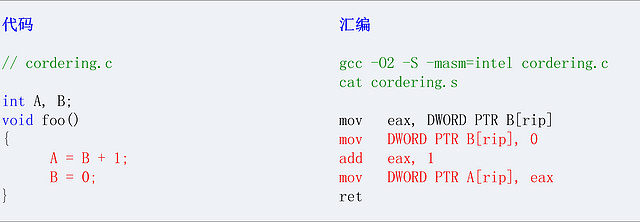
\includegraphics[width=.9\linewidth]{../pic/v6.jpg}
\begin{itemize}
\item 一个简单的示例,全局变量A,B均为非volatile变量。通过gcc O2优化进行编译,你可以惊奇的发现,A,B两个变量的赋值顺序被调换了!!!在对应的汇编代码中,B = 0语句先被执行,然后才是A = B + 1语句被执行。
\item 在这里,我先简单的介绍一下C/C++编译器最基本优化原理:保证一段程序的输出,在优化前后无变化。将此原理应用到上面,可以发现,虽然gcc优化了A,B变量的赋值顺序,但是foo()函数的执行结果,优化前后没有发生任何变化,仍旧是A = 1;B = 0。因此这么做是可行的。
\end{itemize}
\subsubsection{测试用例六:一个Volatile变量}
\label{sec-9-3-2}
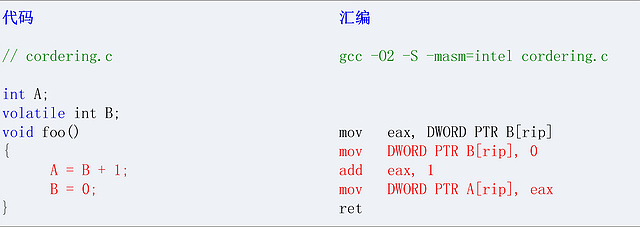
\includegraphics[width=.9\linewidth]{../pic/v7.jpg}
\begin{itemize}
\item 此测试,相对于测试用例五,最大的区别在于,变量B被声明为volatile变量。通过查看对应的汇编代码,B仍旧被提前到A之前赋值,Volatile变量B,并未阻止编译器优化的发生,编译后仍旧发生了乱序现象。
\item 如此看来,C/C++ Volatile变量,与非Volatile变量之间的操作,是可能被编译器交换顺序的。
\item 通过此用例,已经能够很好的说明,本章节前面,通过flag == true,来假设something一定完成是不成立的。在多线程下,如此使用volatile,会产生很严重的问题。但是,这不是终点,请继续看下面的测试用例七。
\end{itemize}
\subsubsection{测试用例七:两个Volatile变量}
\label{sec-9-3-3}
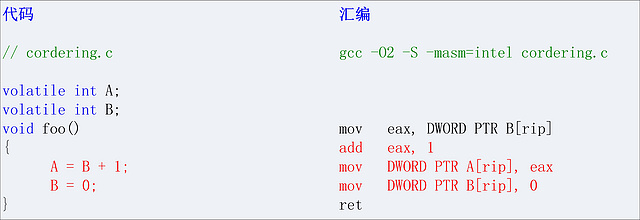
\includegraphics[width=.9\linewidth]{../pic/v8.jpg}
\begin{itemize}
\item 同时将A,B两个变量都声明为volatile变量,再来看看对应的汇编。奇迹发生了,A,B赋值乱序的现象消失。此时的汇编代码,与用户代码顺序高度一直,先赋值变量A,然后赋值变量B。
\item 如此看来,C/C++ Volatile变量间的操作,是不会被编译器交换顺序的。
\end{itemize}
\subsubsection{happens-before}
\label{sec-9-3-4}
\begin{itemize}
\item 通过测试用例六,可以总结出:C/C++ Volatile变量与非Volatile变量间的操作顺序,有可能被编译器交换。因此,上面多线程操作的伪代码,在实际运行的过程中,就有可能变成下面的顺序:

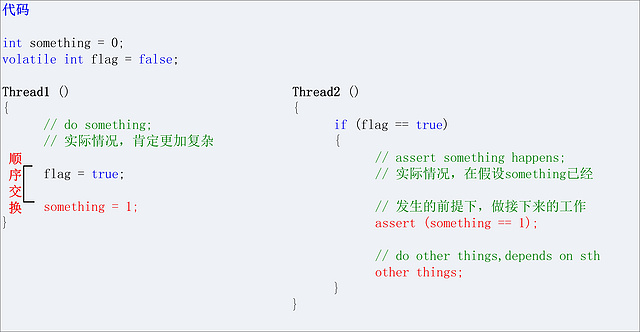
\includegraphics[width=.9\linewidth]{../pic/v9.jpg}

\item 由于Thread1中的代码执行顺序发生变化,flag = true被提前到something之前进行,那么整个Thread2的假设全部失效。由于something未执行,但是Thread2进入了if代码段,整个多线程代码逻辑出现问题,导致多线程完全错误。
\item 细心的读者看到这里,可能要提问,根据测试用例七,C/C++ Volatile变量间,编译器是能够保证不交换顺序的,那么能不能将something中所有的变量全部设置为volatile呢?这样就阻止了编译器的乱序优化,从而也就保证了这个多线程程序的正确性。
\item 针对此问题,很不幸,仍旧不行。将所有的变量都设置为volatile,首先能够阻止编译器的乱序优化,这一点是可以肯定的。但是,别忘了,编译器编译出来的代码,最终是要通过CPU来执行的。目前,市场上有各种不同体系架构的CPU产品,CPU本身为了提高代码运行的效率,也会对代码的执行顺序进行调整,这就是所谓的CPU Memory Model (CPU内存模型)。关于CPU的内存模型,可以参考这些资料:Memory Ordering From Wiki;Memory Barriers Are Like Source Control Operations From Jeff Preshing;CPU Cache and Memory Ordering From 何登成。下面,是截取自Wiki上的一幅图,列举了不同CPU架构,可能存在的指令乱序。

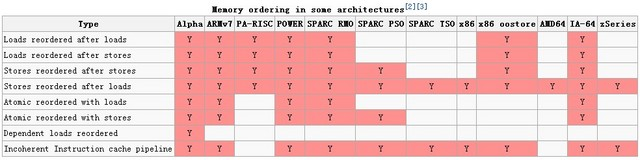
\includegraphics[width=.9\linewidth]{../pic/v10.jpg}

\item 从图中可以看到,X86体系(X86,AMD64),也就是我们目前使用最广的CPU,也会存在指令乱序执行的行为:StoreLoad乱序,读操作可以提前到写操作之前进行。
\item 因此,回到上面的例子,哪怕将所有的变量全部都声明为volatile,哪怕杜绝了编译器的乱序优化,但是针对生成的汇编代码,CPU有可能仍旧会乱序执行指令,导致程序依赖的逻辑出错,volatile对此无能为力。
\item 其实,针对这个多线程的应用,真正正确的做法,是构建一个happens-before语义。关于happens-before语义的定义,可参考文章:The Happens-Before Relation。下面,用图的形式,来展示happens-before语义:

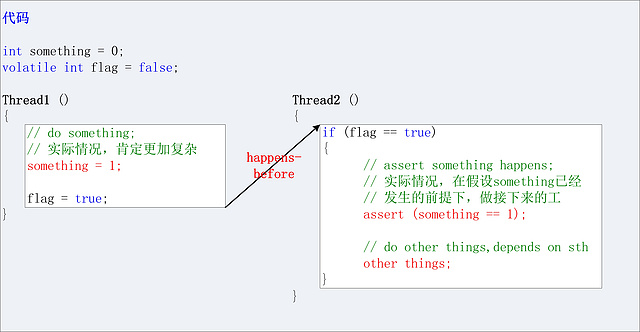
\includegraphics[width=.9\linewidth]{../pic/v11.jpg}

\item 如图所示,所谓的happens-before语义,就是保证Thread1代码块中的所有代码,一定在Thread2代码块的第一条代码之前完成。当然,构建这样的语义有很多方法,我们常用的Mutex、Spinlock、RWLock,都能保证这个语义 (关于happens-before语义的构建,以及为什么锁能保证happens-before语义,以后专门写一篇文章进行讨论)。但是,C/C++ Volatile关键词不能保证这个语义,也就意味着C/C++ Volatile关键词,在多线程环境下,如果使用的不够细心,就会产生如同我这里提到的错误。
\end{itemize}
\subsubsection{小结}
\label{sec-9-3-5}
\begin{itemize}
\item C/C++ Volatile关键词的第三个特性:”顺序性”,能够保证Volatile变量间的顺序性,编译器不会进行乱序优化。Volatile变量与非Volatile变量的顺序,编译器不保证顺序,可能会进行乱序优化。同时,C/C++ Volatile关键词,并不能用于构建happens-before语义,因此在进行多线程程序设计时,要小心使用volatile,不要掉入volatile变量的使用陷阱之中。
\end{itemize}
\subsection{Volatile:Java增强}
\label{sec-9-4}
\begin{itemize}
\item 在介绍了C/C++ Volatile关键词之后,再简单介绍一下Java的Volatile。与C/C++的Volatile关键词类似,Java的Volatile也有这三个特性,但最大的不同在于:第三个特性,”顺序性”,Java的Volatile有很极大的增强,Java Volatile变量的操作,附带了Acquire与Release语义。所谓的Acquire与Release语义,可参考文章:Acquire and Release Semantics。(这一点,后续有必要的话,可以写一篇文章专门讨论)。Java Volatile所支持的Acquire、Release语义,如下:
\item 对于Java Volatile变量的写操作,带有Release语义,所有Volatile变量写操作之前的针对其他任何变量的读写操作,都不会被编译器、CPU优化后,乱序到Volatile变量的写操作之后执行。
\item 对于Java Volatile变量的读操作,带有Acquire语义,所有Volatile变量读操作之后的针对其他任何变量的读写操作,都不会被编译器、CPU优化后,乱序到Volatile变量的读操作之前进行。
\item 通过Java Volatile的Acquire、Release语义,对比C/C++ Volatile,可以看出,Java Volatile对于编译器、CPU的乱序优化,限制的更加严格了。Java Volatile变量与非Volatile变量的一些乱序操作,也同样被禁止。
\item 由于Java Volatile支持Acquire、Release语义,因此Java Volatile,能够用来构建happens-before语义。也就是说,前面提到的C/C++ Volatile在多线程下错误的使用场景,在Java语言下,恰好就是正确的。如下图所示:

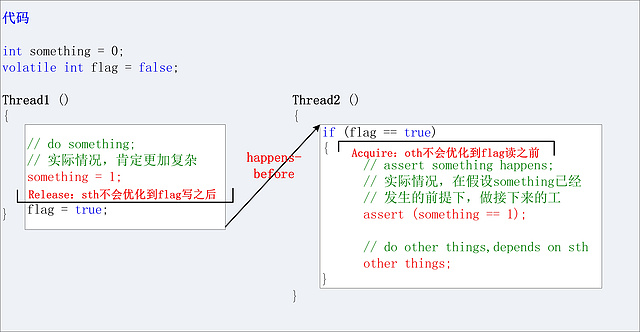
\includegraphics[width=.9\linewidth]{../pic/v12.jpg}
\end{itemize}
\subsection{Volatile的起源}
\label{sec-9-5}
\begin{itemize}
\item C/C++的Volatile关键词,有三个特性:易变性;不可优化性;顺序性。那么,为什么Volatile被设计成这样呢?要回答这个问题,就需要从Volatile关键词的产生说起。(注:这一小节的内容,参考自C++ and the Perils of Double-Checked Locking论文的第10章节:volatile:A Brief History。这是一篇顶顶好的论文,值得多次阅读,强烈推荐!)
\item Volatile关键词,最早出现于19世纪70年代,被用于处理memory-mapeed I/O (MMIO)带来的问题。在引入MMIO之后,一块内存地址,既有可能是真正的内存,也有可能被映射到一个I/O端口。相对的,读写一个内存地址,既有可能操作内存,也有可能读写的是一个I/O设备。MMIO为什么需要引入Volatile关键词?考虑如下的一个代码片段:

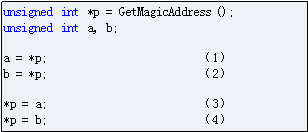
\includegraphics[width=.9\linewidth]{../pic/v13.png}

\item 在此代码片段中,指针p既有可能指向一个内存地址,也有可能指向一个I/O设备。如果指针p指向的是I/O设备,那么(1),(2)中的a,b,就会接收到I/O设备的连续两个字节。但是,p也有可能指向内存,此时,编译器的优化策略,就可能会判断出a,b同时从同一内存地址读取数据,在做完(1)之后,直接将a赋值给b。对于I/O设备,需要防止编译器做这个优化,不能假设指针b指向的内容不变——易变性。
\item 同样,代码(3),(4)也有类似的问题,编译器发现将a,b同时赋值给指针p是无意义的,因此可能会优化代码(3)中的赋值操作,仅仅保留代码(4)。对于I/O设备,需要防止编译器将写操作给彻底优化消失了——”不可优化”性。
\item 对于I/O设备,编译器不能随意交互指令的顺序,因为顺序一变,写入I/O设备的内容也就发生变化了——”顺序性”。
\item 基于MMIO的这三个需求,设计出来的C/C++ Volatile关键词,所含有的特性,也就是本文前面分析的三个特性:易变性;不可优化性;顺序性。
\end{itemize}

\section{QT中实现Thread与GUI主线程连通方法}
\label{sec-10}
\url{http://mobile.51cto.com/symbian-270684.htm}

\section{Other Reference}
\label{sec-11}
\begin{itemize}
\item 了解 Qt 多线程编程 新手必学(1)
\end{itemize}
\url{http://mobile.51cto.com/symbian-269482.htm}
\begin{itemize}
\item QT核心编程之Qt线程 (3)
\end{itemize}
\url{http://mobile.51cto.com/symbian-270589.htm}
\begin{itemize}
\item 浅谈Qt中多线程编程
\end{itemize}
\url{http://mobile.51cto.com/symbian-268343.htm}
\begin{itemize}
\item 解析 QT 多线程程序详细设计 上篇
\end{itemize}
\url{http://mobile.51cto.com/symbian-270667.htm}
\begin{itemize}
\item 解析QT多线程程序详细设计之QObject可重入性 下篇
\end{itemize}
\url{http://mobile.51cto.com/symbian-270674.htm}
\begin{itemize}
\item Qt的插件机制(1)
\end{itemize}
\url{http://mobile.51cto.com/symbian-268027.htm}
\begin{itemize}
\item Qt和KDE在未来将面临新的挑战和机遇
\end{itemize}
\url{http://mobile.51cto.com/hot-247522.htm}
\begin{itemize}
\item QT源码之Qt信号槽机制与事件机制的联系
\end{itemize}
\url{http://mobile.51cto.com/symbian-270997.htm}
\begin{itemize}
\item QT进程间通信 详细介绍
\end{itemize}
\url{http://mobile.51cto.com/symbian-270726.htm}
\begin{itemize}
\item 解析 QT 静态库和动态库
\end{itemize}
\url{http://mobile.51cto.com/symbian-267846.htm}
\begin{itemize}
\item Linux下 QT 实现串口通讯小实例
\end{itemize}
\url{http://mobile.51cto.com/symbian-270754.htm}
\begin{itemize}
\item Linux 虚拟串口及 Qt 串口通信实例
\end{itemize}
\url{http://mobile.51cto.com/symbian-270768.htm}
\begin{itemize}
\item TTY 驱动
\end{itemize}
\url{http://oss.org.cn/kernel-book/ldd3/ch18.html}
\begin{itemize}
\item 
\item 
\item 
\item 
\item 
\item 
\item 
\item 
\item 
\item 
\item 
\item 
\item 
\end{itemize}
% Emacs 24.3.1 (Org mode 8.2.7c)
\end{document}